% Customizable fields and text areas start with % >> below.
% Lines starting with the comment character (%) are normally removed before release outside the collaboration, but not those comments ending lines

% svn info. These are modified by svn at checkout time.
% The last version of these macros found before the maketitle will be the one on the front page,
% so only the main file is tracked.
% Do not edit by hand!
\RCS$Revision: 110744 $
\RCS$HeadURL: svn+ssh://svn.cern.ch/reps/tdr2/notes/AN-12-008/trunk/AN-12-008.tex $
\RCS$Id: AN-12-008.tex 110744 2012-03-15 00:17:51Z dudero $
%%%%%%%%%%%%% local definitions %%%%%%%%%%%%%%%%%%%%%
% This allows for switching between one column and two column (cms@external) layouts
% The widths should  be modified for your particular figures. You'll need additional copies if you have more than one standard figure size.
\newlength\cmsFigWidth
\ifthenelse{\boolean{cms@external}}{\setlength\cmsFigWidth{0.85\columnwidth}}{\setlength\cmsFigWidth{0.4\textwidth}}
\ifthenelse{\boolean{cms@external}}{\providecommand{\cmsLeft}{top}}{\providecommand{\cmsLeft}{left}}
\ifthenelse{\boolean{cms@external}}{\providecommand{\cmsRight}{bottom}}{\providecommand{\cmsRight}{right}}
%%%%%%%%%%%%%%%  Title page %%%%%%%%%%%%%%%%%%%%%%%%
\cmsNoteHeader{AN-12-008} % This is over-written in the CMS environment: useful as preprint no. for export versions
% >> Title: please make sure that the non-TeX equivalent is in PDFTitle below
\title{Multivariate optimization and background estimation for the Standard Model Higgs boson search in H$\to$WW$\to\ell\nu jj$ decay}

% >> Authors
%Author is always "The CMS Collaboration" for PAS and papers, so author, etc, below will be ignored in those cases
%For multiple affiliations, create an address entry for the combination


\address[ttu]{Texas Tech University, Lubbock, Texas, USA}
\address[fnal]{Fermi National Accelerator Laboratory, Batavia, Illinois, USA}
\address[tamu]{Texas A\&M University, College Station, Texas, USA}
\address[nebr]{University of Nebraska at Lincoln, Nebraska, USA}
\address[uerj]{Universidade do Estado do Rio de Janeiro (UERJ), Brazil}

\author[ttu]{Nural~Akchurin}
\author[fnal]{Jake~Anderson}
\author[fnal]{Andrew Beretvas}
\author[fnal]{Jeffrey~Berryhill}
\author[fnal]{Pushpa~Bhat}
\author[ttu]{Phil~Dudero}
\author[tamu]{Ricardo~Eusebi}
\author[fnal]{Dan~Green}
\author[nebr]{Pratima~Jindal}
\author[ttu]{Sung-Won Lee}
\author[fnal]{Kalanand~Mishra}
\author[tamu]{Ilya~Osipenkov}
\author[tamu]{Alexx~Perloff}
\author[uerj]{Andre~Sznajder}
\author[fnal]{Nhan~V.~Tran}
\author[fnal]{Fan~Yang}
\author[fnal]{Francisco~Yumiceva}


% >> Date
% The date is in yyyy/mm/dd format. Today has been
% redefined to match, but if the date needs to be fixed, please write it in this fashion.
% For papers and PAS, \today is taken as the date the head file (this one) was last modified according to svn: see the RCS Id string above.
% For the final version it is best to "touch" the head file to make sure it has the latest date.
\date{\today}

% >> Abstract
% Abstract processing:
% 1. **DO NOT use \include or \input** to include the abstract: our abstract extractor will not search through other files than this one.
% 2. **DO NOT use %**                  to comment out sections of the abstract: the extractor will still grab those lines (and they won't be comments any longer!).
% 3. **DO NOT use tex macros**         in the abstract: External TeX parsers used on the abstract don't understand them.
\abstract{
We present a study of the multi-variate optimization
for the Higgs boson search in the H$\to$WW$\to\ell\nu jj$
final state in the gluon fusion production mechanism. 
Using a complete set of mostly uncorrelated variables 
we optimize each Higgs mass points separately to distinguish 
between the Higgs signal and the dominant W+jets background.
We also develop a data-driven technique to derive 4-body 
$m_{\ell\nu jj}$ invariant mass shape for W+jets background. 
For this we use events in the upper and lower sidebands 
of the $m_{jj}$ distribution to extract the 4-body mass 
shape for events in the signal region  
65 GeV ~$< m_{jj} <$~95 GeV. 
Using this data-driven technique we are able to keep 
the systematic uncertainties (dominated by background 
shape systematics) to within a few percent. 
This analysis note complements the documentation of the 
main analysis in AN-11/110.
}

% >> PDF Metadata
% Do not comment out the following hypersetup lines (metadata). They will disappear in NODRAFT mode and are needed by CDS.
% Also: make sure that the values of the metadata items are sensible and are in plain text (no TeX! -- for \sqrt{s} use sqrt(s) -- this will show with extra quote marks in the draft version but is okay).

\hypersetup{%
pdfauthor={Jake Anderson, Phil Dudero, 
Pratima Jindal, Kalanand Mishra, Ilya Osipenkov, Fan Yang},%
pdftitle={Multivariate optimization and background estimation for the Standard Model Higgs boson search in HtoWWtoellnujj decay},%
pdfsubject={CMS},%
pdfkeywords={CMS, physics, software, computing}}

\maketitle %maketitle comes after all the front information has been supplied

% >> Text
%%%%%%%%%%%%%%%%%%%%%%%%%%%%%%%%  Begin text %%%%%%%%%%%%%%%%%%%%%%%%%%%%%
%% **DO NOT REMOVE THE BIBLIOGRAPHY** which is located before the appendix.
%% You can take the text between here and the bibiliography as an example which you should replace with the actual text of your document.
%% If you include other TeX files, be sure to use "\input{filename}" rather than "\input filename".
%% The latter works for you, but our parser looks for the braces and will break when uploading the document.
%%%%%%%%%%%%%%%
\tableofcontents
\newpage
\section{Introduction}

In the present iteration of the analysis our goal is to 
reconstruct either a linear discriminant or likelihood of 
minimum number of uncorrelated variables necessary to 
describe the event topology. 
This is because the individual cuts are highly 
inefficient. 
To keep the analysis as simple as possible we have intentionally 
not focused on exploiting the full potential of the 
multivariate analysis because this would involve 
inclusion of additional correlated variables.



\subsection{Training and validation method}
The Toolkit for Multivariate Data Analysis with ROOT 
(TMVA)~\cite{tmva}
is a toolkit to be implemented using ROOT that allows the user 
to carry out a significant number of multivariate analysis 
techniques such as boosted decision trees, neural networks, 
projected likelihood estimators and linear discriminants.

Using TMVA to implement the majority of these techniques 
consists of two phases: the Training Phase and the Testing Phase. 
To begin the Training Phase, the user must have samples where 
it is known which events are to be classified as signal and which 
are to be classified as background. 
Using this information, TMVA is trained to separate these classes 
as efficiently as possible. 
Next, the Testing Phase simply stands to implement the trained 
method of separation on a dataset where it is unknown which 
events are to be classified as signal or background. 

In the present analysis we try three classifiers to separate 
Higgs signal from the background: linear discriminant (LD),
likelihood, and boosted decision tree (BDT).
We have tried to use a complete set of minimum number of 
input variables necessary to describe the whole event topology, 
as will be described in detail in the next section.


The TMVA has some knobs to optimize the
performance of various classifiers, but we didn't tune these knobs. 
In the region of interest to us (90--95\% background
rejection points) the likelihood and BDT classifiers have almost 
identical performance. 
This is expected because the input variables are mostly uncorrelated, 
and there are no large correlations to be exploited.

We have also seen in the previous iterations of training that
with inclusion of additional (correlated) variables the BDT
performs better than likelihood. However, some of these
variables were correlated with the 4-body mass ($m_{WW} = m_{\ell\nu jj}$), 
so we decided to trim down to the minimum possible complete
set comprising of 10 variables. 


\subsection{Training and validation samples}
We perform a two-component multivariate analysis (MVA) to 
separate the Higgs signal from the dominant W+jets background.
We used the Fall11 MC samples for both Higgs signal and the 
W+jets background, as listed in Table~\ref{tab:MCsamples}.
%%%%%%%%%%%%%%%%%%%%%%%%%%
\begin{table}[htb]
  \begin{center}
    \begin{tabular}{l|l} 
      \hline
       Category & Sample name\\
      \hline
      Background & {\footnotesize /WJetsToLNu\_TuneZ2\_7TeV-madgraph-tauola/Fall11-PU\_S6\_START42\_V14B-v1/AODSIM}  \\
      \hline
      Signal &  {\footnotesize /GluGluToHToWWToLNuQQ\_M-*\_7TeV-powheg-pythia6/Fall11-PU\_S6\_START42\_}\\
       &  {\footnotesize V14B-v1/AODSIM} (with Higgs mass from 170 to 600~GeV) \\
      \hline
    \end{tabular}
  \end{center}
  \caption{Summary of Monte Carlo training and testing samples used in the analysis. 
    We use 50\% of the events in each category for training and the other 50\% for testing/validation.}
  \label{tab:MCsamples}
\end{table}
%%%%%%%%%%%%%%%%%%%%%%%%%%

\subsection{Training method}
We train the MVA separately for the following 12 Higgs mass 
points: 170, 180, 190, 200, 250, 300, 350, 400, 450, 500, 550, and 600~GeV.
Exactly 50\% of the events in each category are used for training 
the classifier and the other 50\% are used for testing/validation.
We train separately the events with two jets 
and three jets in the final state, because the background composition 
and kinematics are different for the two categories.
We also train separately for the two lepton species, \textit{i.e.}, 
muons and electrons.
In the following sections we will show the plots for muon channel 
only because the corresponding plots for the electron channel are 
very similar.


\subsection{Selection cuts}
Selection cuts are identical to the pre-selection described in 
CMS AN-2011/110. These include requirements on lepton ID, loose 
jet ID, second lepton veto in the event, and minimum missing transverse 
energy (25 GeV for muon and 35 GeV for electron events). 


\newpage
\section{Input variables used for MVA training}
In this section we outline the inputs that are used to discriminate between the 
SM Higgs signal and the dominant $W$ + jets background.  
The inputs are combined into a multivariate discriminant in order to maximize the 
separation.  
To describe the process at leading order, the maximal set of observables is given by~\cite{Gao:2010qx,Dobrescu:2009zf}:
\begin{equation}
\{ m_{l\nu jj}, m_{jj}, \cos\theta_1, \cos\theta_2, \Phi, \cos\theta^{\ast}, \Phi_1 \}
\end{equation}
The invariant mass of the leptonic $W$, $m_{l\nu}$, is constrained in the kinematic fit to compute the longitudinal momentum 
of the neutrino.  The angular variables are correlated and defined in Fig.~\ref{fig:anglesWWlvjj}.
%%%%%%%%%%%%%%%%%%%
\begin{figure}[ht]
  \centering
  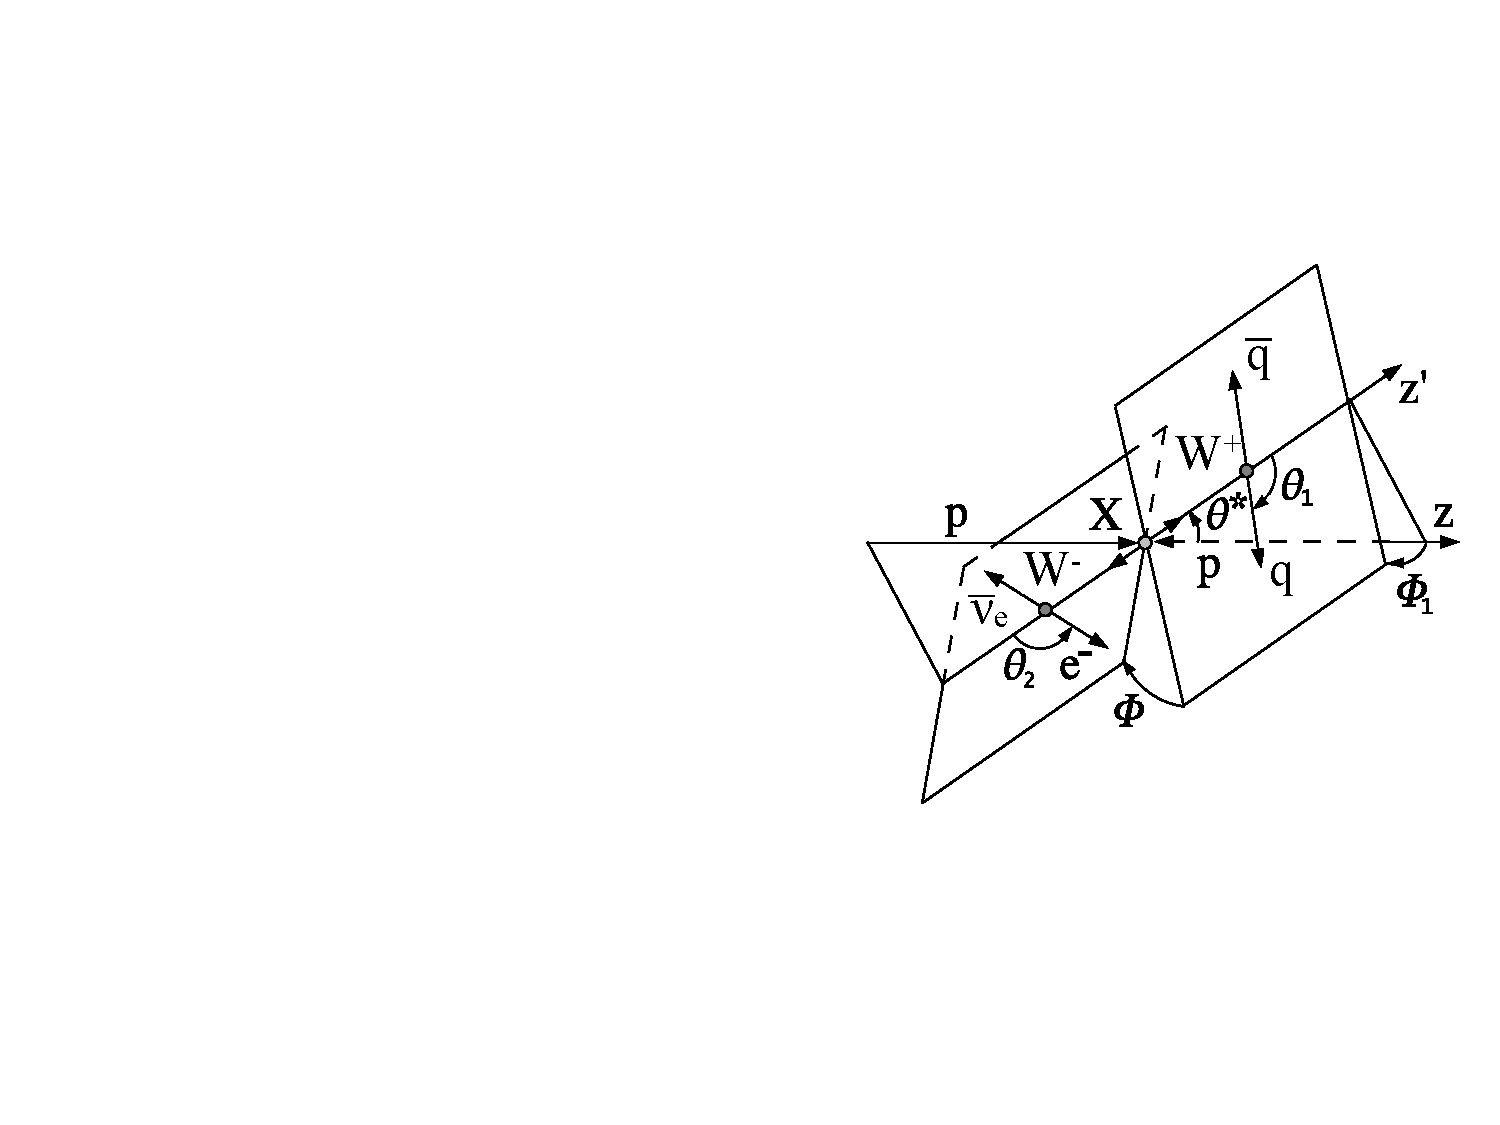
\includegraphics[width=0.5\textwidth]{figs/angles_wwlvjj.pdf}
  \caption{\label{fig:anglesWWlvjj}Angular definition for the $WW\to l\nu jj$ process}
\end{figure}
%%%%%%%%%%%%%%%%%%%
The angle $\cos\theta^{\ast}$ is the polar angle between the parton collision axis z and the $X$ 
decay axis $z'$, both defined in the $X$ rest frame. The angle $\Phi_1$ is the azimuthal angle
between the $zz'$ plane and the decay plane of hadronic $W$. The angles 
$\cos\theta^{\ast}$ and $\Phi_1$ are denoted as production
angles because they depend on the production mechanism, $gg$ or $q\bar{q}$.
For the SM Higgs which is a spin-zero particle, the production angles are flat (before acceptance). 
The angle $\Phi$ is the angle between the decay planes of the two $W$ systems in the $X$ rest
frame. The angle $\theta_i$ is the angle between
the direction of the fermion f from $W \to f\bar{f}$ and the direction opposite the $X$ in
the $W_i$ rest frame, where index i = 1, 2 refers to the first or second $W$ boson. 
In the case of the $\cos\theta_i$ angle from the hadronic $W$, it is ambiguous as to which jet is originating from the 
fermion or anti-fermion, so the angles is defined from $0$ to $\pi$ for the leading $p_T$ jet.  
Finally, The angles $\Phi$, $\cos\theta_1$ and $\cos\theta_2$ do not depend on the production mechanism and are denoted as the helicity angles.

The observables $m_{l\nu jj}$ and $m_{jj}$ are excluded from the MVA inputs.
The observable, $m_{l\nu jj}$, is not used because it is the distribution of this observable which is used
in the extraction of the upper limit.
The observable, $m_{jj}$, is not used since the $m_{jj}$ distribution is used to extract from the sideband to the signal region
to extract a data-driven shape for the background in the $m_{l\nu jj}$ spectrum. 
The leaves the five angular variables as inputs to the multivariate discriminant.  
As an example, the related search for the Higgs in the $ZZ \to 2l2q$ final state at CMS~\cite{CMS2l2q} uses these five observables
in an angular discriminant. 
Since the invariant masses are not used in the multivariate discriminant, the angular variables are defined in a loose window in 
$m_{l\nu jj}$ in order to take into account the correlations between the angles and the masses.  

In addition, to the five angular variables the $p_T$ of the WW system $p_{T,WW}$ 
and longitudinal boost (rapidity) $Y_{WW}$ are also used.  
The $Y_{WW}$ distribution comes from the parton distribution functions. 
The $p_{T,WW}$ distribution comes from next-to-leading order effects.  
The lepton charge is also included to give some discrimination power since the $W$ + jets background 
is asymmetric with respect to charge while the SM Higgs signal will be symmetric in lepton charge.  
These two quantities in addition to the mass and angular quantities form a full set of kinematic observables for process.
Other discriminating observables such as the $p_T$ of the $W\to jj$ system are not independent of the full set 
(and particularly of $m_{l\nu jj}$ and $m_{jj}$) are thus not used since they can sculpt the invariant mass distributions
to make the background more "signal-like".

%%Finally the quark-gluon likelihood discriminant observables for the two jets are used.  
%%The quark-gluon likelihood discriminant gives a measure of a jet originating from a quark or gluon~\cite{qgAN}
%%The SM Higgs signal consists of quark jets while the background is an admixture of both quark and gluon jets.  
%%
Combining all the inputs together the final set of inputs to the multivariate discriminant is:
\begin{equation}
\{ \cos\theta_1, \cos\theta_2, \Phi, \cos\theta^{\ast}, \Phi_1, p_{T,WW}, Y_{WW}, {\rm lepton~charge}\}
\end{equation}
%As an example, we plot the input variables for the SM Higgs mass of 300~GeV for the 2-jet $W\to\mu\nu$ category in Fig.~\ref{fig:inputs3002jmu}.


The distributions of input variables are shown in Figs~\ref{fig:inputs1702jmu}--\ref{fig:inputs6003jmu}
for various Higgs mass points and jet multiplicities.
%%%%%%%%%%%%%%%%%%%
\subsection{Input variables: \texorpdfstring{$M_H$}{M(H)} = 170~GeV, 2 jets}
%%%%%%%%%%%%%%%%%%%
\begin{figure}[ht]
  \centering
  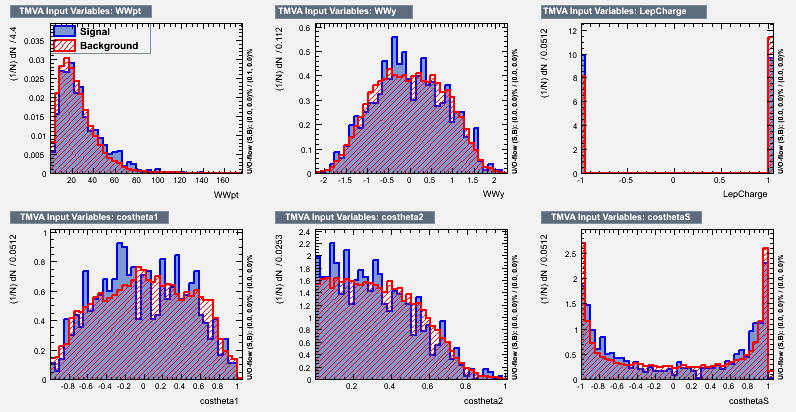
\includegraphics[width=0.8\textwidth]{figs/TMVA_170_nJ2_mu_variables_id_c1.png}
  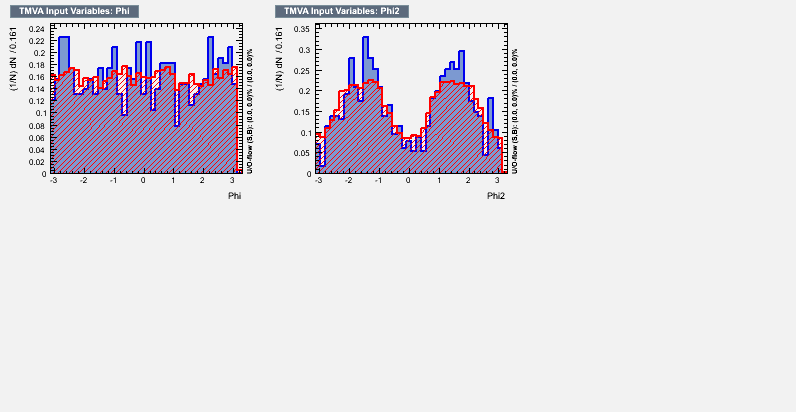
\includegraphics[width=0.8\textwidth]{figs/TMVA_170_nJ2_mu_variables_id_c2.png}	
  \caption{\label{fig:inputs1702jmu}Inputs to the multivariate discriminant for SM Higgs mass of 170~GeV for the 2-jet $W\to\mu\nu$ category}
\end{figure}
%%%%%%%%%%%%%%%%%%%
\newpage
\subsection{Input variables: \texorpdfstring{$M_H$}{M(H)} = 170~GeV, 3 jets}
%%%%%%%%%%%%%%%%%%%
\begin{figure}[ht]
  \centering
  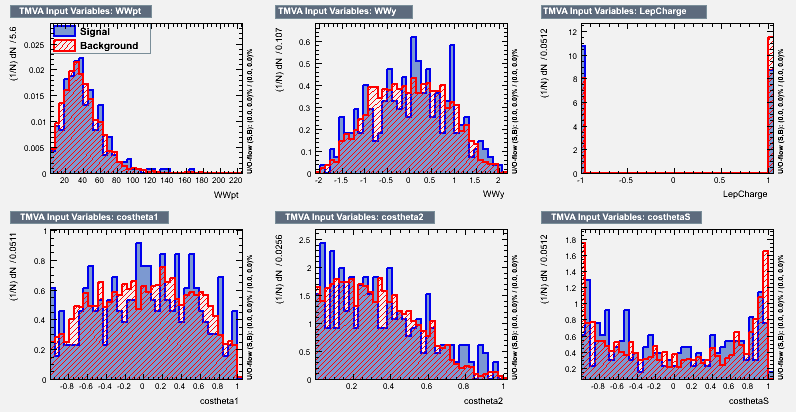
\includegraphics[width=0.8\textwidth]{figs/TMVA_170_nJ3_mu_variables_id_c1.png}
  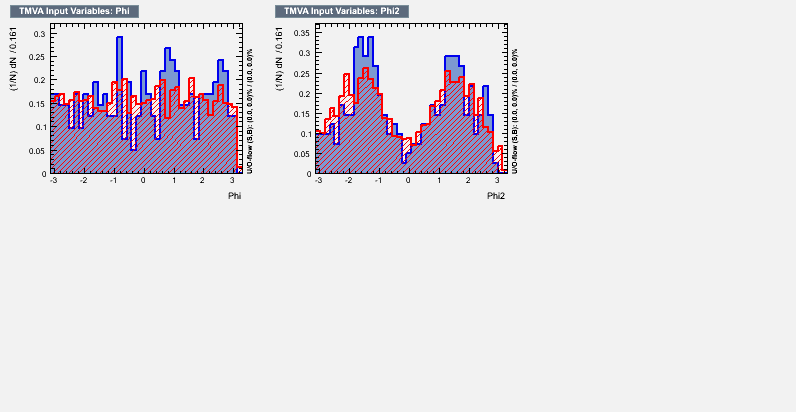
\includegraphics[width=0.8\textwidth]{figs/TMVA_170_nJ3_mu_variables_id_c2.png}	
  \caption{\label{fig:inputs1703jmu}Inputs to the multivariate discriminant for SM Higgs mass of 170~GeV for the 3-jet $W\to\mu\nu$ category}
\end{figure}
%%%%%%%%%%%%%%%%%%%
\newpage
\subsection{Input variables: \texorpdfstring{$M_H$}{M(H)} = 180~GeV, 2 jets}
%%%%%%%%%%%%%%%%%%%
\begin{figure}[ht]
  \centering
  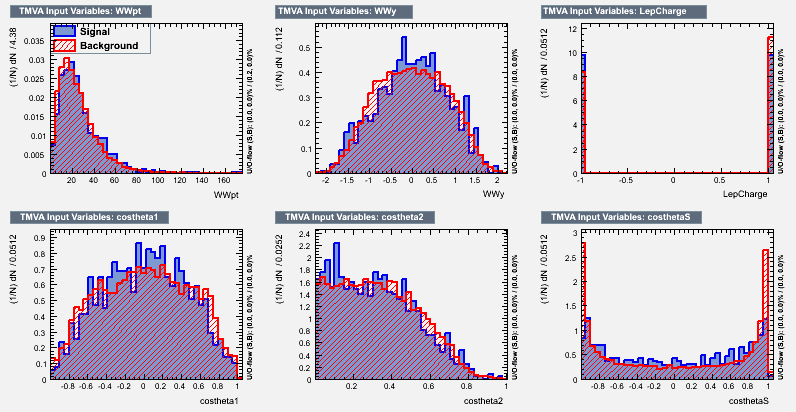
\includegraphics[width=0.8\textwidth]{figs/TMVA_180_nJ2_mu_variables_id_c1.png}
  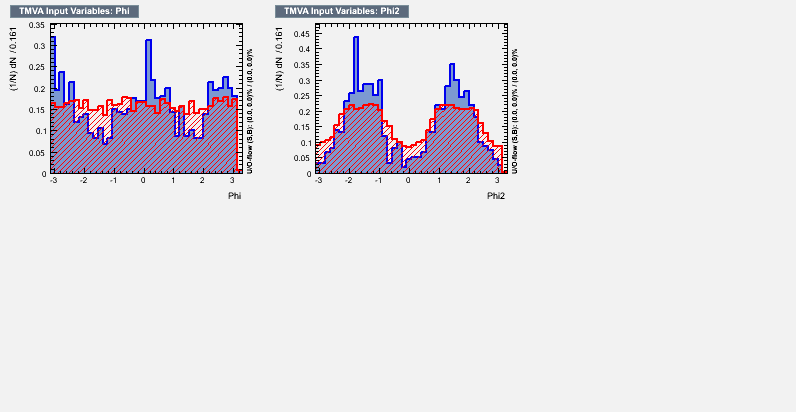
\includegraphics[width=0.8\textwidth]{figs/TMVA_180_nJ2_mu_variables_id_c2.png}	
  \caption{\label{fig:inputs1802jmu}Inputs to the multivariate discriminant for SM Higgs mass of 180~GeV for the 2-jet $W\to\mu\nu$ category}
\end{figure}
%%%%%%%%%%%%%%%%%%%
\newpage
\subsection{Input variables: \texorpdfstring{$M_H$}{M(H)} = 180~GeV, 3 jets}
%%%%%%%%%%%%%%%%%%%
\begin{figure}[ht]
  \centering
  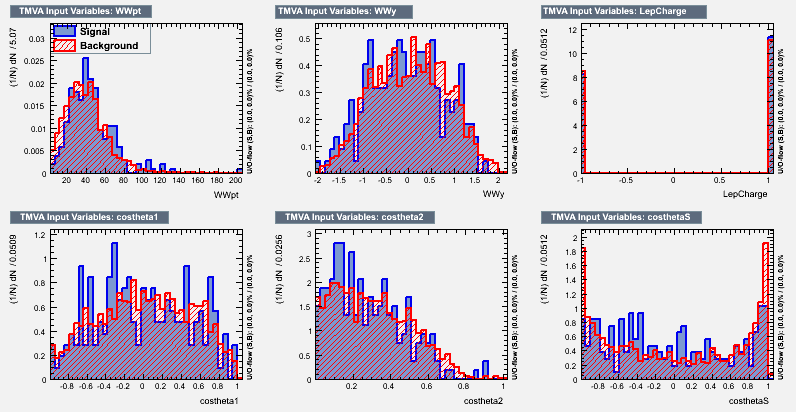
\includegraphics[width=0.8\textwidth]{figs/TMVA_180_nJ3_mu_variables_id_c1.png}
  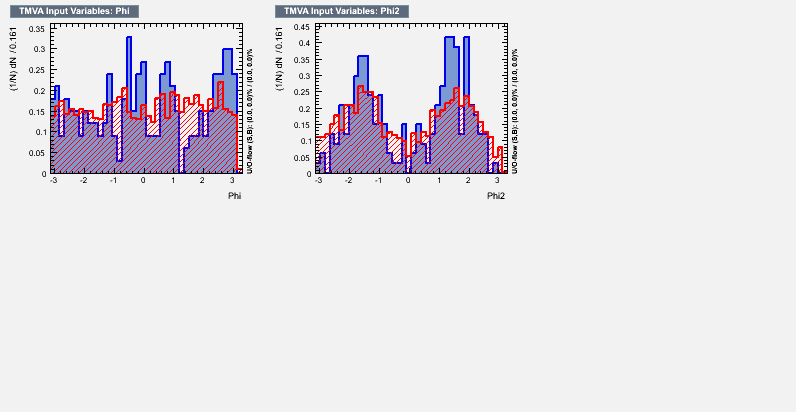
\includegraphics[width=0.8\textwidth]{figs/TMVA_180_nJ3_mu_variables_id_c2.png}	
  \caption{\label{fig:inputs1803jmu}Inputs to the multivariate discriminant for SM Higgs mass of 180~GeV for the 3-jet $W\to\mu\nu$ category}
\end{figure}
%%%%%%%%%%%%%%%%%%%
\newpage
\subsection{Input variables: \texorpdfstring{$M_H$}{M(H)} = 190~GeV, 2 jets}
%%%%%%%%%%%%%%%%%%%
\begin{figure}[ht]
  \centering
  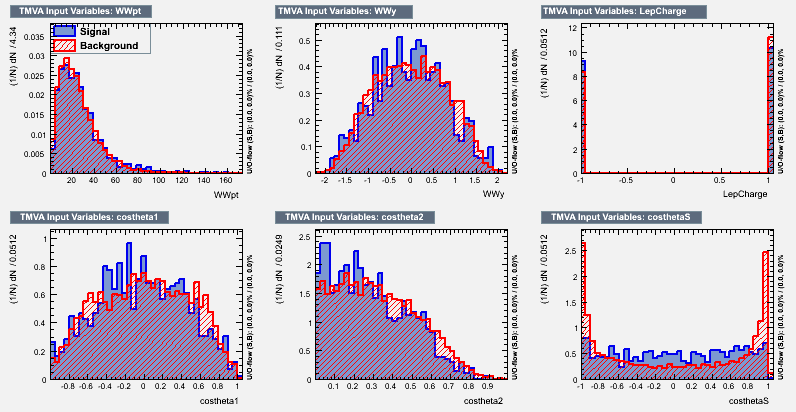
\includegraphics[width=0.8\textwidth]{figs/TMVA_190_nJ2_mu_variables_id_c1.png}
  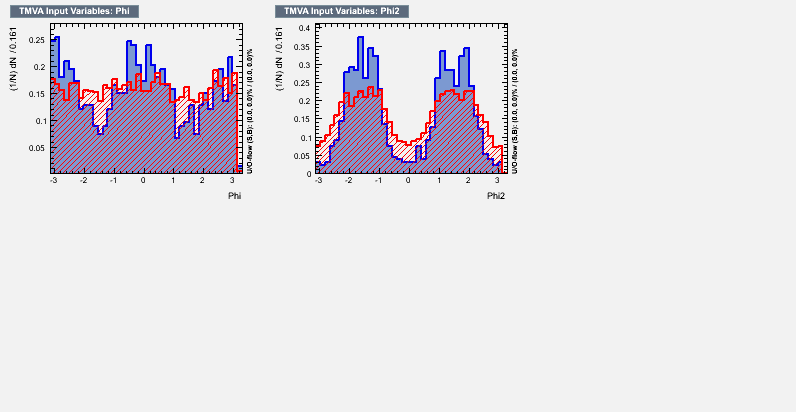
\includegraphics[width=0.8\textwidth]{figs/TMVA_190_nJ2_mu_variables_id_c2.png}	
  \caption{\label{fig:inputs1902jmu}Inputs to the multivariate discriminant for SM Higgs mass of 190~GeV for the 2-jet $W\to\mu\nu$ category}
\end{figure}
%%%%%%%%%%%%%%%%%%%
\newpage
\subsection{Input variables: \texorpdfstring{$M_H$}{M(H)} = 190~GeV, 3 jets}
%%%%%%%%%%%%%%%%%%%
\begin{figure}[ht]
  \centering
  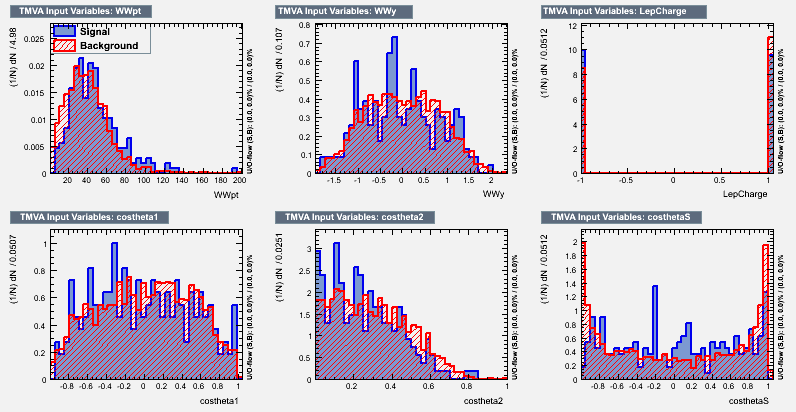
\includegraphics[width=0.8\textwidth]{figs/TMVA_190_nJ3_mu_variables_id_c1.png}
  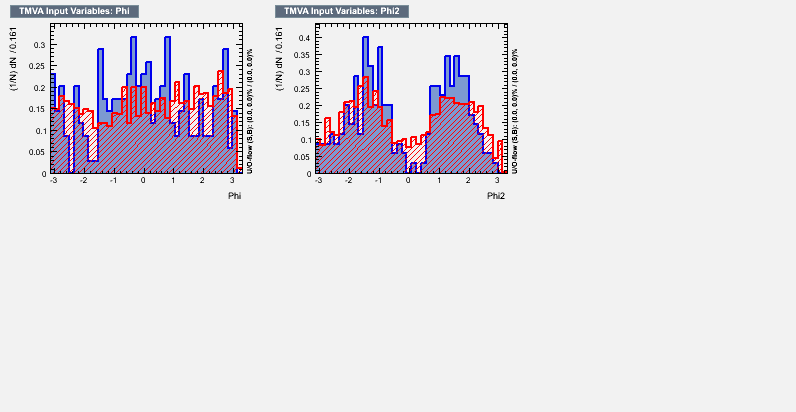
\includegraphics[width=0.8\textwidth]{figs/TMVA_190_nJ3_mu_variables_id_c2.png}	
  \caption{\label{fig:inputs1903jmu}Inputs to the multivariate discriminant for SM Higgs mass of 190~GeV for the 3-jet $W\to\mu\nu$ category}
\end{figure}
%%%%%%%%%%%%%%%%%%%
\newpage
\subsection{Input variables: \texorpdfstring{$M_H$}{M(H)} = 200~GeV, 2 jets}
%%%%%%%%%%%%%%%%%%%
\begin{figure}[ht]
  \centering
  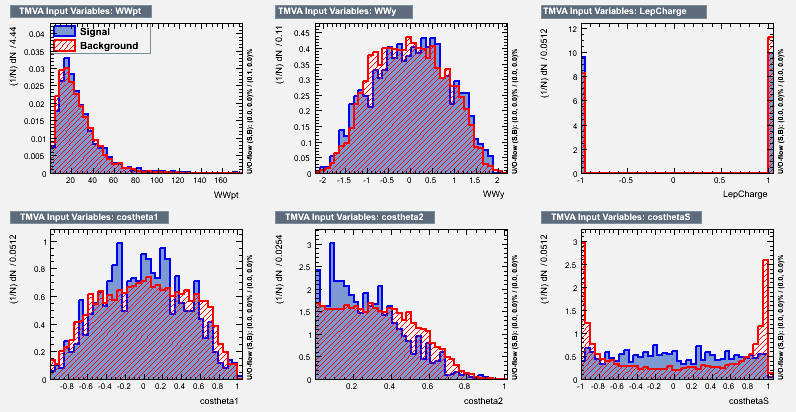
\includegraphics[width=0.8\textwidth]{figs/TMVA_200_nJ2_mu_variables_id_c1.png}
  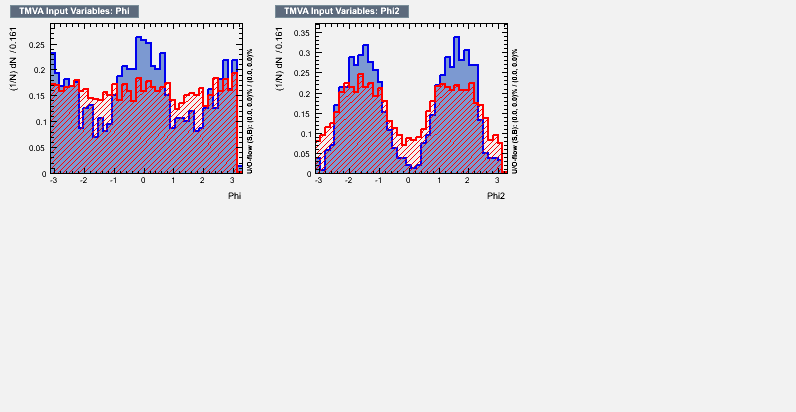
\includegraphics[width=0.8\textwidth]{figs/TMVA_200_nJ2_mu_variables_id_c2.png}	
  \caption{\label{fig:inputs2002jmu}Inputs to the multivariate discriminant for SM Higgs mass of 200~GeV for the 2-jet $W\to\mu\nu$ category}
\end{figure}
%%%%%%%%%%%%%%%%%%%
\newpage
\subsection{Input variables: \texorpdfstring{$M_H$}{M(H)} = 200~GeV, 3 jets}
%%%%%%%%%%%%%%%%%%%
\begin{figure}[ht]
  \centering
  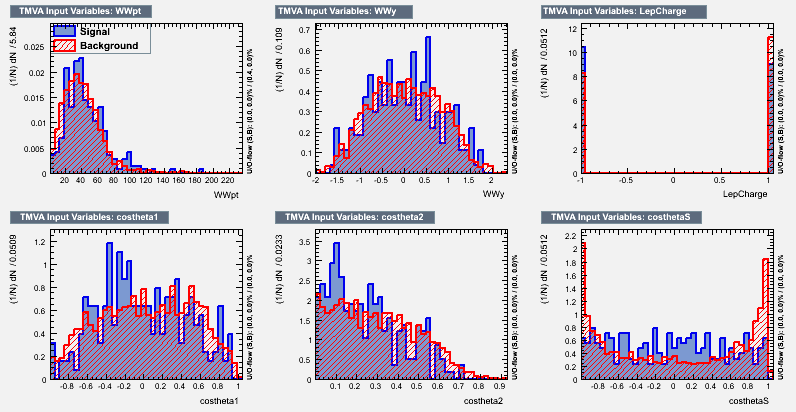
\includegraphics[width=0.8\textwidth]{figs/TMVA_200_nJ3_mu_variables_id_c1.png}
  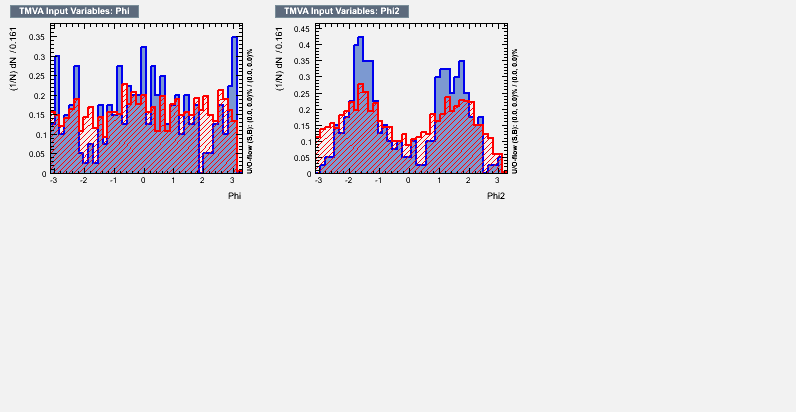
\includegraphics[width=0.8\textwidth]{figs/TMVA_200_nJ3_mu_variables_id_c2.png}	
  \caption{\label{fig:inputs2003jmu}Inputs to the multivariate discriminant for SM Higgs mass of 200~GeV for the 3-jet $W\to\mu\nu$ category}
\end{figure}
%%%%%%%%%%%%%%%%%%%
\newpage
\subsection{Input variables: \texorpdfstring{$M_H$}{M(H)} = 250~GeV, 2 jets}
%%%%%%%%%%%%%%%%%%%
\begin{figure}[ht]
  \centering
  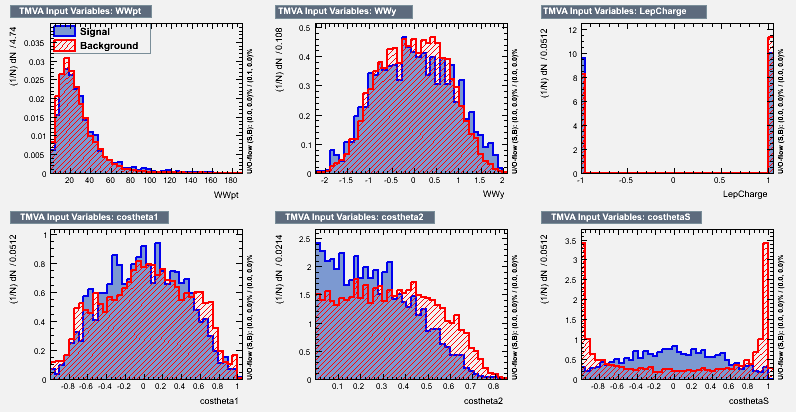
\includegraphics[width=0.8\textwidth]{figs/TMVA_250_nJ2_mu_variables_id_c1.png}
  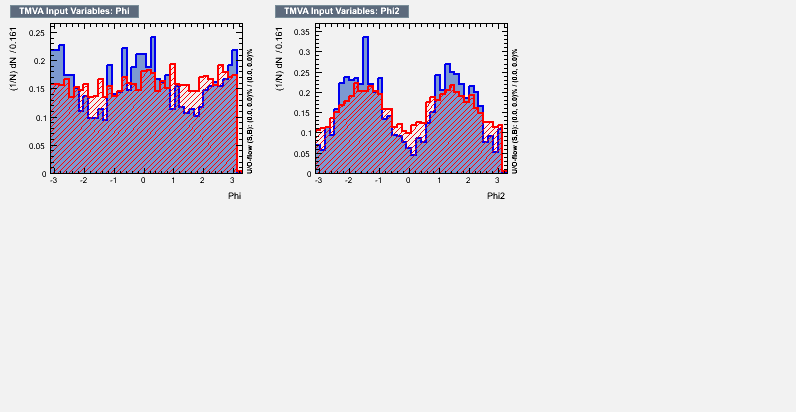
\includegraphics[width=0.8\textwidth]{figs/TMVA_250_nJ2_mu_variables_id_c2.png}	
  \caption{\label{fig:inputs2502jmu}Inputs to the multivariate discriminant for SM Higgs mass of 250~GeV for the 2-jet $W\to\mu\nu$ category}
\end{figure}
%%%%%%%%%%%%%%%%%%%
\newpage
\subsection{Input variables: \texorpdfstring{$M_H$}{M(H)} = 250~GeV, 3 jets}
%%%%%%%%%%%%%%%%%%%
\begin{figure}[ht]
  \centering
  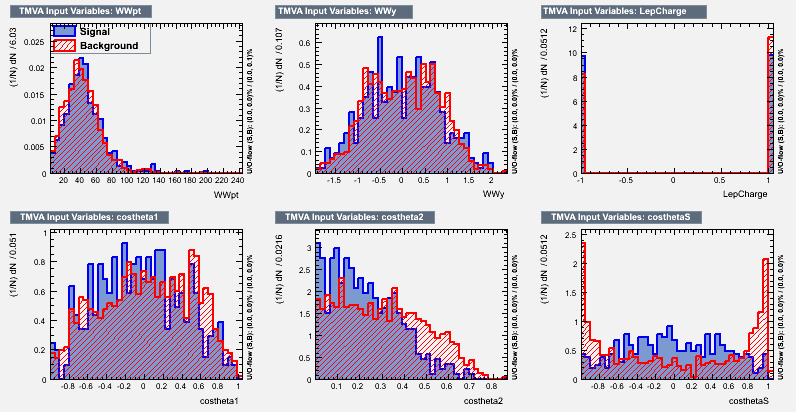
\includegraphics[width=0.8\textwidth]{figs/TMVA_250_nJ3_mu_variables_id_c1.png}
  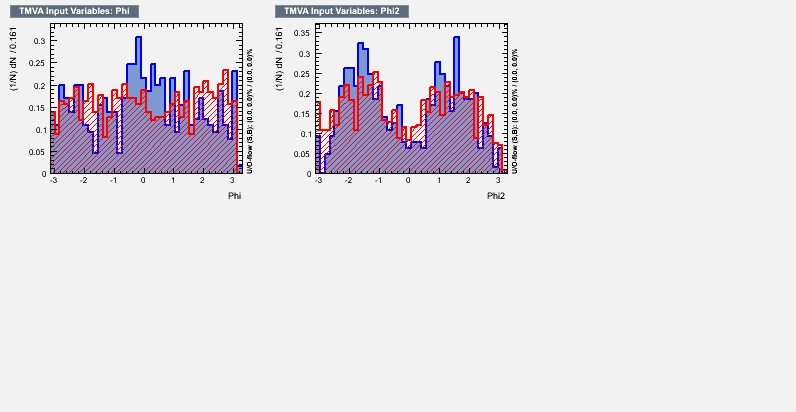
\includegraphics[width=0.8\textwidth]{figs/TMVA_250_nJ3_mu_variables_id_c2.png}	
  \caption{\label{fig:inputs2503jmu}Inputs to the multivariate discriminant for SM Higgs mass of 250~GeV for the 3-jet $W\to\mu\nu$ category}
\end{figure}
%%%%%%%%%%%%%%%%%%%
\newpage
\subsection{Input variables: \texorpdfstring{$M_H$}{M(H)} = 300~GeV, 2 jets}
%%%%%%%%%%%%%%%%%%%
\begin{figure}[ht]
  \centering
  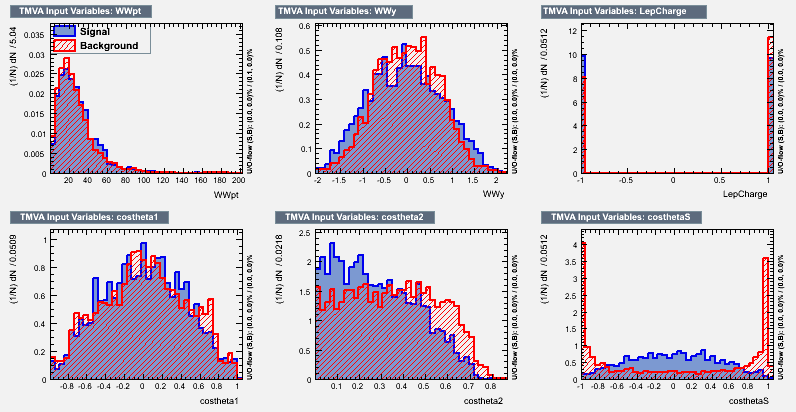
\includegraphics[width=0.8\textwidth]{figs/TMVA_300_nJ2_mu_variables_id_c1.png}
  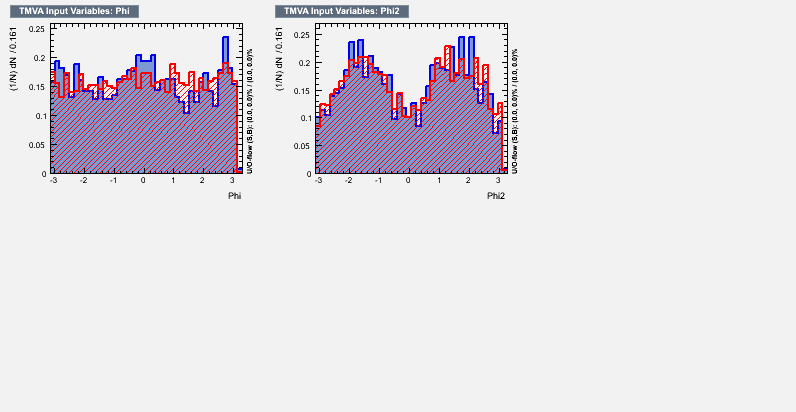
\includegraphics[width=0.8\textwidth]{figs/TMVA_300_nJ2_mu_variables_id_c2.png}	
  \caption{\label{fig:inputs3002jmu}Inputs to the multivariate discriminant for SM Higgs mass of 300~GeV for the 2-jet $W\to\mu\nu$ category}
\end{figure}
%%%%%%%%%%%%%%%%%%%
\newpage
\subsection{Input variables: \texorpdfstring{$M_H$}{M(H)} = 300~GeV, 3 jets}
%%%%%%%%%%%%%%%%%%%
\begin{figure}[ht]
  \centering
  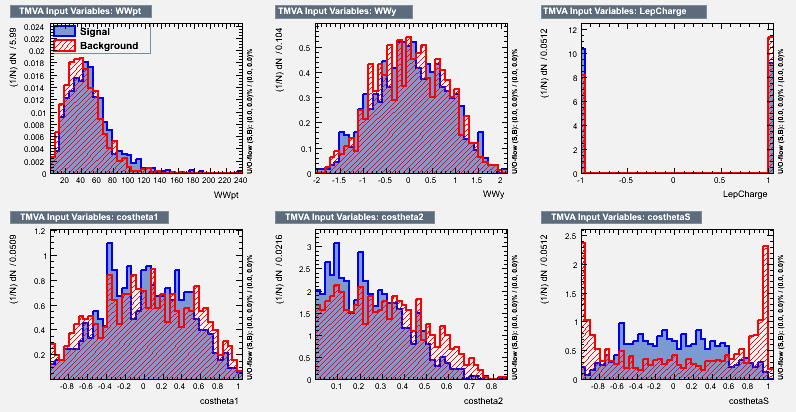
\includegraphics[width=0.8\textwidth]{figs/TMVA_300_nJ3_mu_variables_id_c1.png}
  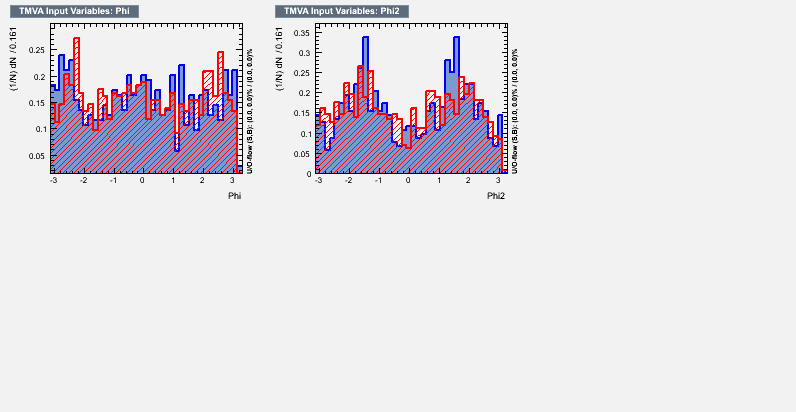
\includegraphics[width=0.8\textwidth]{figs/TMVA_300_nJ3_mu_variables_id_c2.png}	
  \caption{\label{fig:inputs3003jmu}Inputs to the multivariate discriminant for SM Higgs mass of 300~GeV for the 3-jet $W\to\mu\nu$ category}
\end{figure}
%%%%%%%%%%%%%%%%%%%
\newpage
\subsection{Input variables: \texorpdfstring{$M_H$}{M(H)} = 350~GeV, 2 jets}
%%%%%%%%%%%%%%%%%%%
\begin{figure}[ht]
  \centering
  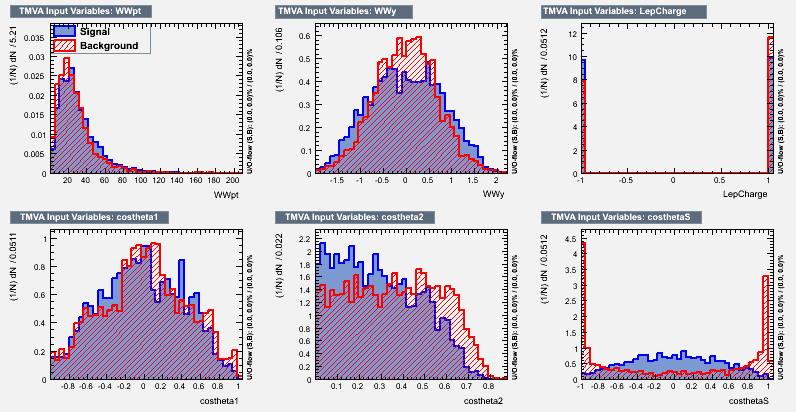
\includegraphics[width=0.8\textwidth]{figs/TMVA_350_nJ2_mu_variables_id_c1.png}
  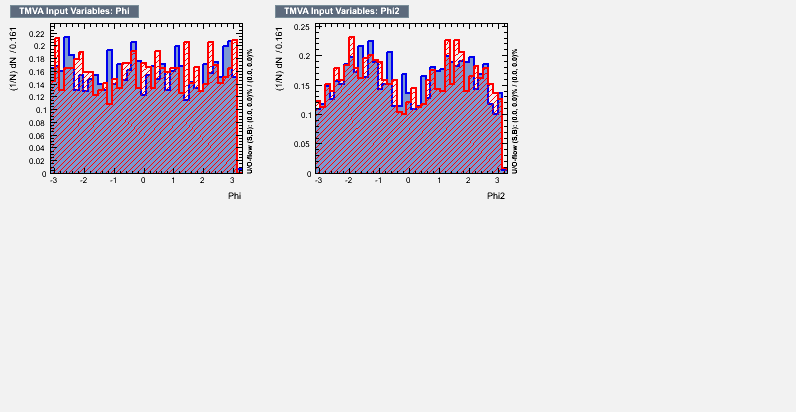
\includegraphics[width=0.8\textwidth]{figs/TMVA_350_nJ2_mu_variables_id_c2.png}	
  \caption{\label{fig:inputs3502jmu}Inputs to the multivariate discriminant for SM Higgs mass of 350~GeV for the 2-jet $W\to\mu\nu$ category}
\end{figure}
%%%%%%%%%%%%%%%%%%%
\newpage
\subsection{Input variables: \texorpdfstring{$M_H$}{M(H)} = 350~GeV, 3 jets}
%%%%%%%%%%%%%%%%%%%
\begin{figure}[ht]
  \centering
  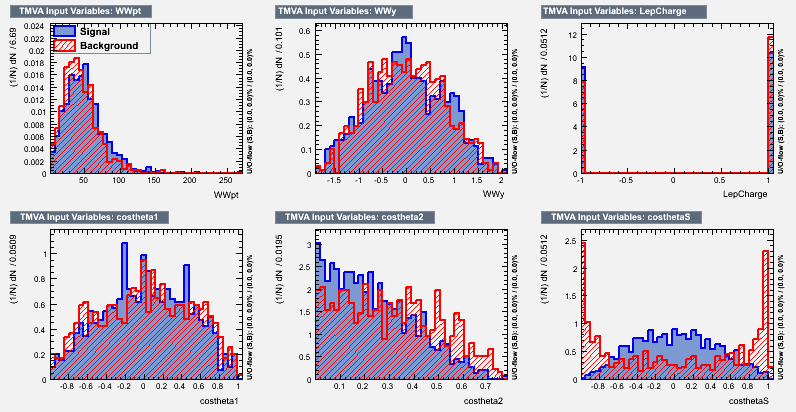
\includegraphics[width=0.8\textwidth]{figs/TMVA_350_nJ3_mu_variables_id_c1.png}
  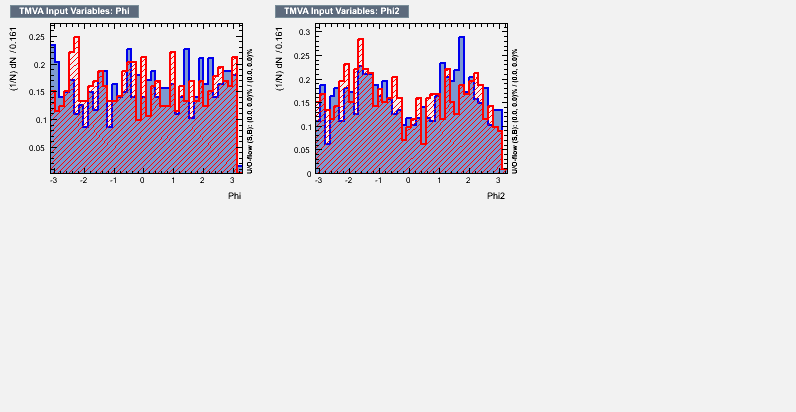
\includegraphics[width=0.8\textwidth]{figs/TMVA_350_nJ3_mu_variables_id_c2.png}	
  \caption{\label{fig:inputs3503jmu}Inputs to the multivariate discriminant for SM Higgs mass of 350~GeV for the 3-jet $W\to\mu\nu$ category}
\end{figure}
%%%%%%%%%%%%%%%%%%%
\newpage
\subsection{Input variables: \texorpdfstring{$M_H$}{M(H)} = 400~GeV, 2 jets}
%%%%%%%%%%%%%%%%%%%
\begin{figure}[ht]
  \centering
  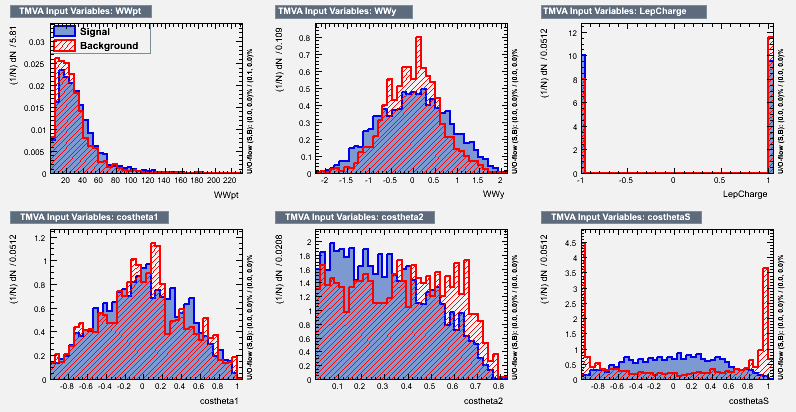
\includegraphics[width=0.8\textwidth]{figs/TMVA_400_nJ2_mu_variables_id_c1.png}
  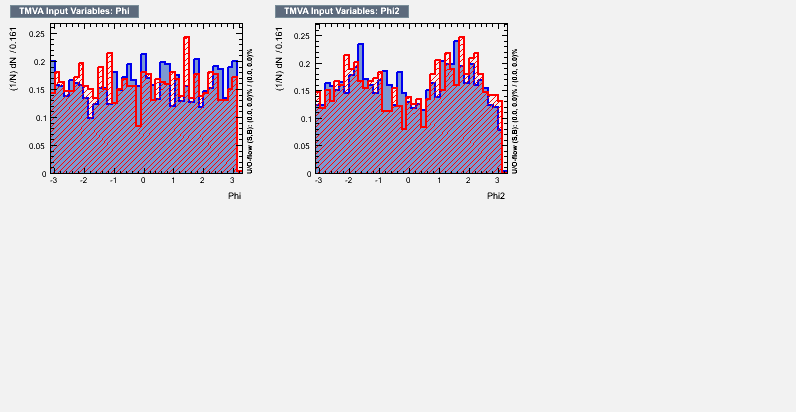
\includegraphics[width=0.8\textwidth]{figs/TMVA_400_nJ2_mu_variables_id_c2.png}	
  \caption{\label{fig:inputs4002jmu}Inputs to the multivariate discriminant for SM Higgs mass of 400~GeV for the 2-jet $W\to\mu\nu$ category}
\end{figure}
%%%%%%%%%%%%%%%%%%%
\newpage
\subsection{Input variables: \texorpdfstring{$M_H$}{M(H)} = 400~GeV, 3 jets}
%%%%%%%%%%%%%%%%%%%
\begin{figure}[ht]
  \centering
  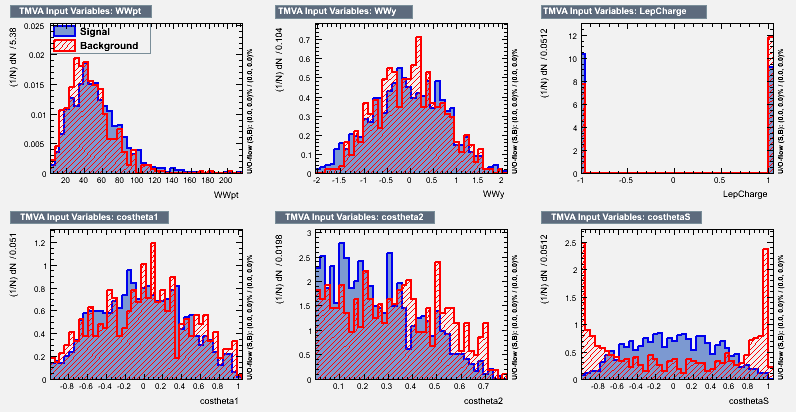
\includegraphics[width=0.8\textwidth]{figs/TMVA_400_nJ3_mu_variables_id_c1.png}
  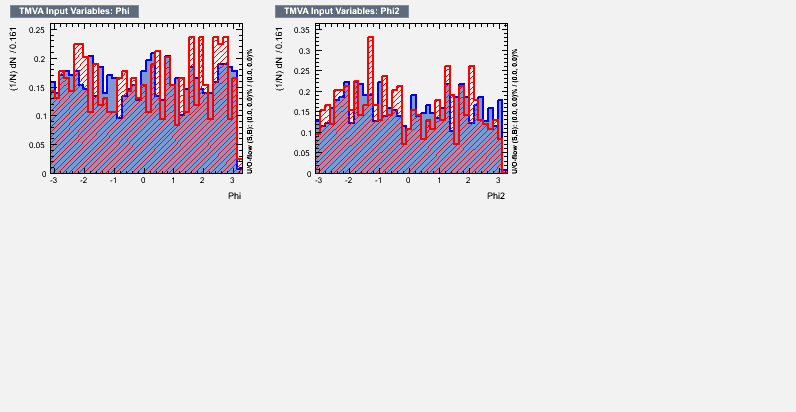
\includegraphics[width=0.8\textwidth]{figs/TMVA_400_nJ3_mu_variables_id_c2.png}	
  \caption{\label{fig:inputs4003jmu}Inputs to the multivariate discriminant for SM Higgs mass of 400~GeV for the 3-jet $W\to\mu\nu$ category}
\end{figure}
%%%%%%%%%%%%%%%%%%%
\newpage
\subsection{Input variables: \texorpdfstring{$M_H$}{M(H)} = 450~GeV, 2 jets}
%%%%%%%%%%%%%%%%%%%
\begin{figure}[ht]
  \centering
  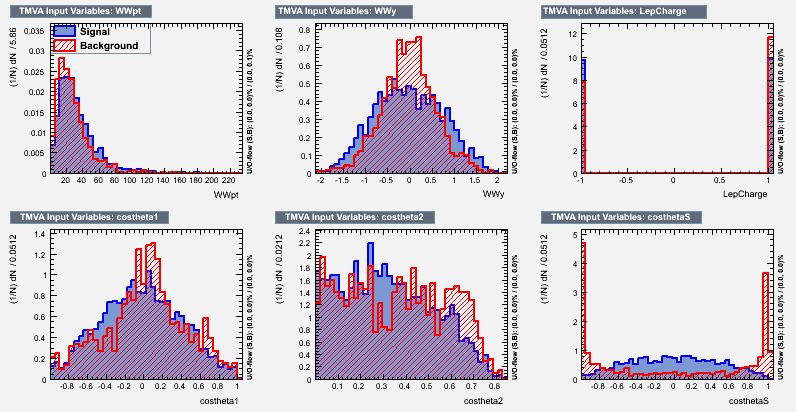
\includegraphics[width=0.8\textwidth]{figs/TMVA_450_nJ2_mu_variables_id_c1.png}
  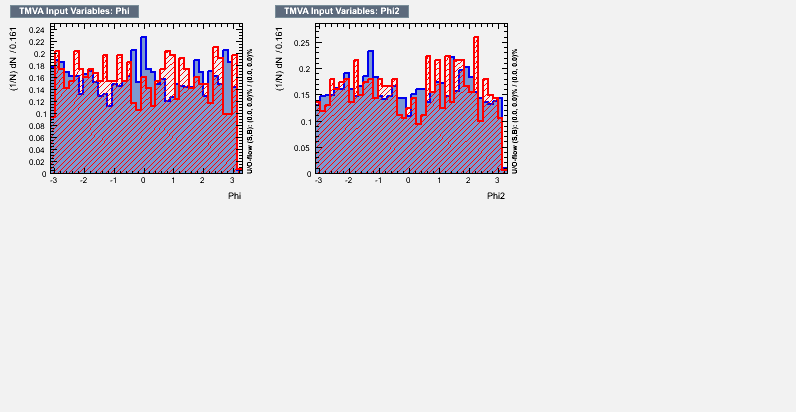
\includegraphics[width=0.8\textwidth]{figs/TMVA_450_nJ2_mu_variables_id_c2.png}	
  \caption{\label{fig:inputs4502jmu}Inputs to the multivariate discriminant for SM Higgs mass of 450~GeV for the 2-jet $W\to\mu\nu$ category}
\end{figure}
%%%%%%%%%%%%%%%%%%%
\newpage
\subsection{Input variables: \texorpdfstring{$M_H$}{M(H)} = 450~GeV, 3 jets}
%%%%%%%%%%%%%%%%%%%
\begin{figure}[ht]
  \centering
  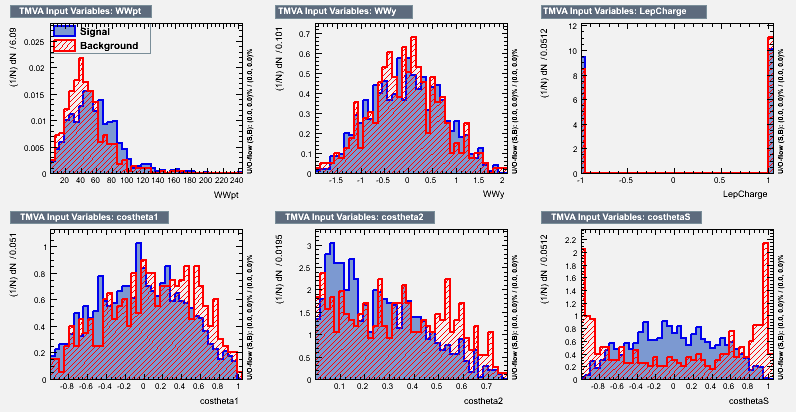
\includegraphics[width=0.8\textwidth]{figs/TMVA_450_nJ3_mu_variables_id_c1.png}
  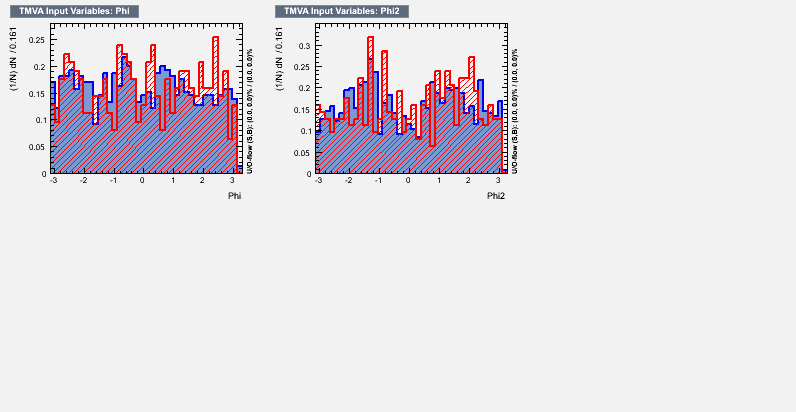
\includegraphics[width=0.8\textwidth]{figs/TMVA_450_nJ3_mu_variables_id_c2.png}	
  \caption{\label{fig:inputs4503jmu}Inputs to the multivariate discriminant for SM Higgs mass of 450~GeV for the 3-jet $W\to\mu\nu$ category}
\end{figure}
%%%%%%%%%%%%%%%%%%%
\newpage
\subsection{Input variables: \texorpdfstring{$M_H$}{M(H)} = 500~GeV, 2 jets}
%%%%%%%%%%%%%%%%%%%
\begin{figure}[ht]
  \centering
  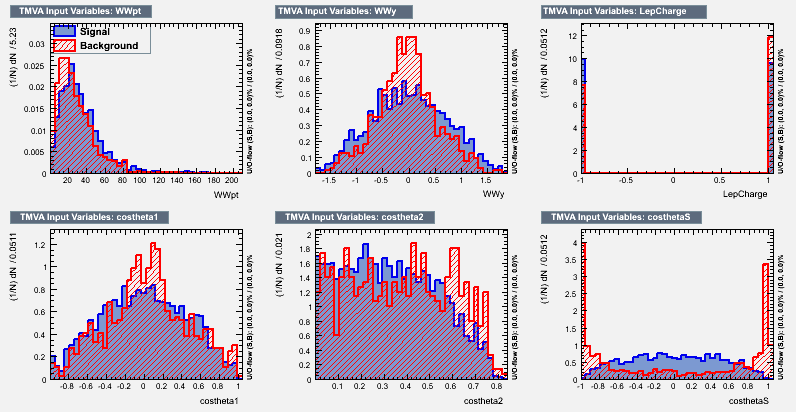
\includegraphics[width=0.8\textwidth]{figs/TMVA_500_nJ2_mu_variables_id_c1.png}
  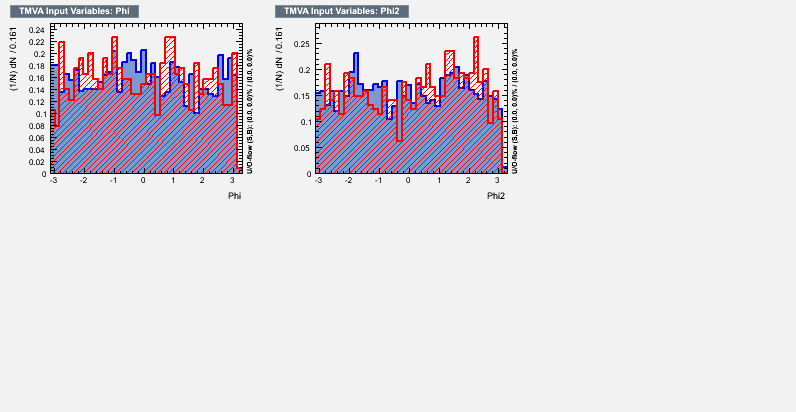
\includegraphics[width=0.8\textwidth]{figs/TMVA_500_nJ2_mu_variables_id_c2.png}	
  \caption{\label{fig:inputs5002jmu}Inputs to the multivariate discriminant for SM Higgs mass of 500~GeV for the 2-jet $W\to\mu\nu$ category}
\end{figure}
%%%%%%%%%%%%%%%%%%%
\newpage
\subsection{Input variables: \texorpdfstring{$M_H$}{M(H)} = 500~GeV, 3 jets}
%%%%%%%%%%%%%%%%%%%
\begin{figure}[ht]
  \centering
  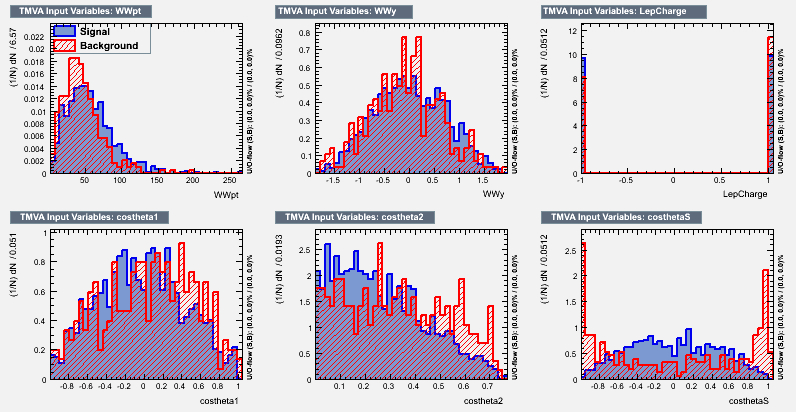
\includegraphics[width=0.8\textwidth]{figs/TMVA_500_nJ3_mu_variables_id_c1.png}
  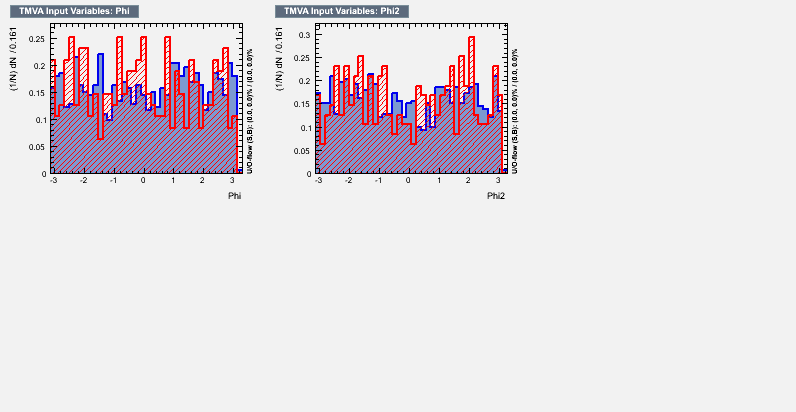
\includegraphics[width=0.8\textwidth]{figs/TMVA_500_nJ3_mu_variables_id_c2.png}	
  \caption{\label{fig:inputs5003jmu}Inputs to the multivariate discriminant for SM Higgs mass of 500~GeV for the 3-jet $W\to\mu\nu$ category}
\end{figure}
%%%%%%%%%%%%%%%%%%%
\newpage
\subsection{Input variables: \texorpdfstring{$M_H$}{M(H)} = 550~GeV, 2 jets}
%%%%%%%%%%%%%%%%%%%
\begin{figure}[ht]
  \centering
  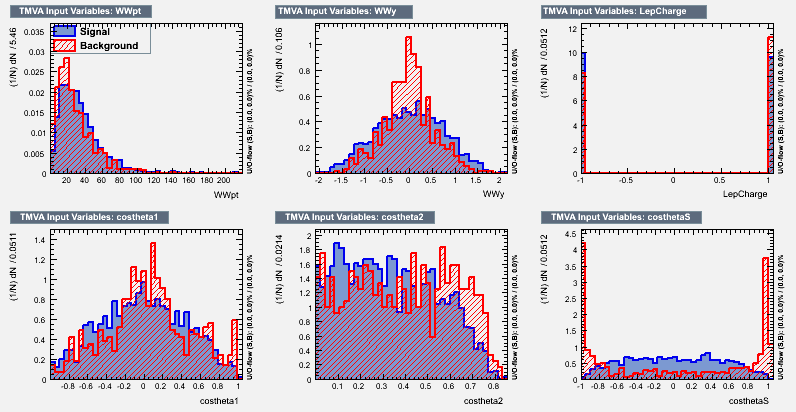
\includegraphics[width=0.8\textwidth]{figs/TMVA_550_nJ2_mu_variables_id_c1.png}
  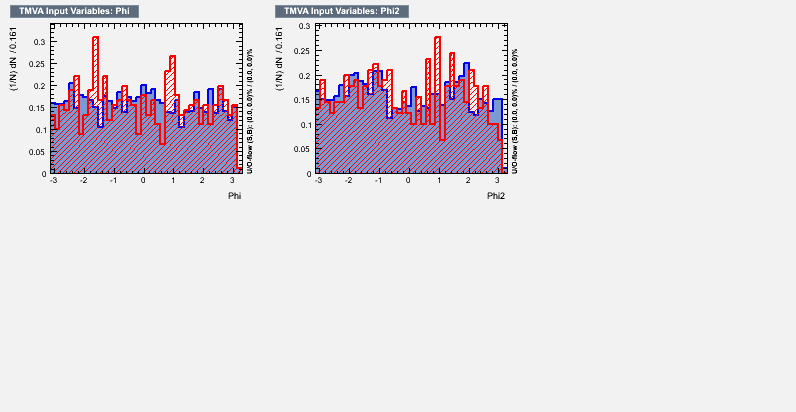
\includegraphics[width=0.8\textwidth]{figs/TMVA_550_nJ2_mu_variables_id_c2.png}	
  \caption{\label{fig:inputs5502jmu}Inputs to the multivariate discriminant for SM Higgs mass of 550~GeV for the 2-jet $W\to\mu\nu$ category}
\end{figure}
%%%%%%%%%%%%%%%%%%%
\newpage
\subsection{Input variables: \texorpdfstring{$M_H$}{M(H)} = 550~GeV, 3 jets}
%%%%%%%%%%%%%%%%%%%
\begin{figure}[ht]
  \centering
  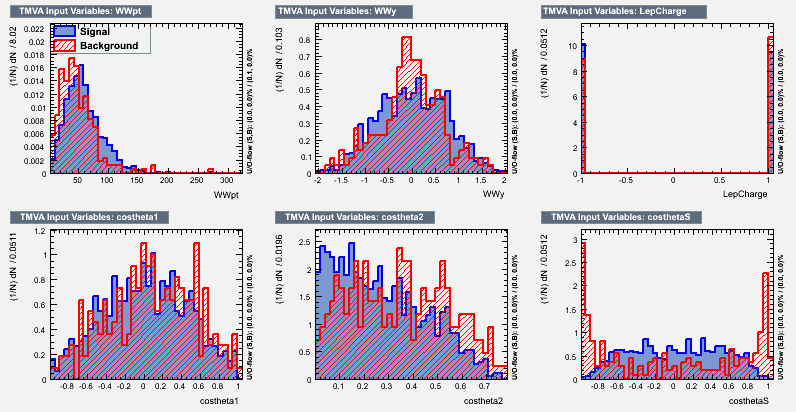
\includegraphics[width=0.8\textwidth]{figs/TMVA_550_nJ3_mu_variables_id_c1.png}
  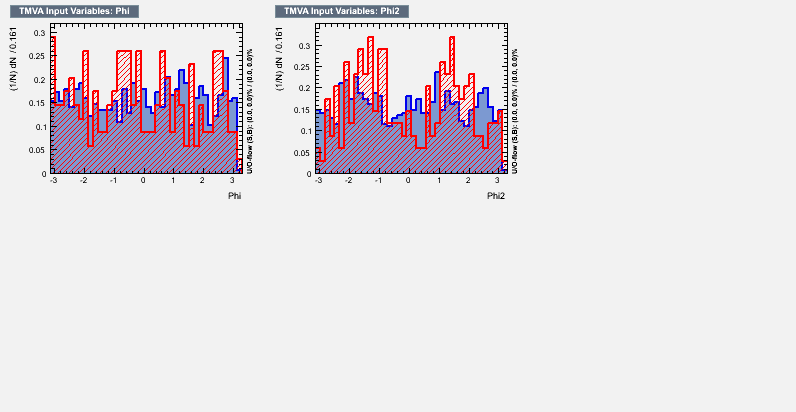
\includegraphics[width=0.8\textwidth]{figs/TMVA_550_nJ3_mu_variables_id_c2.png}	
  \caption{\label{fig:inputs5503jmu}Inputs to the multivariate discriminant for SM Higgs mass of 550~GeV for the 3-jet $W\to\mu\nu$ category}
\end{figure}
%%%%%%%%%%%%%%%%%%%
\newpage
\subsection{Input variables: \texorpdfstring{$M_H$}{M(H)} = 600~GeV, 2 jets}
%%%%%%%%%%%%%%%%%%%
\begin{figure}[ht]
  \centering
  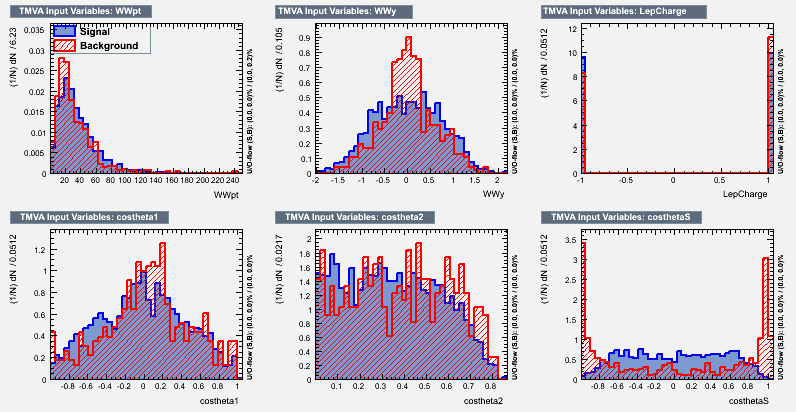
\includegraphics[width=0.8\textwidth]{figs/TMVA_600_nJ2_mu_variables_id_c1.png}
  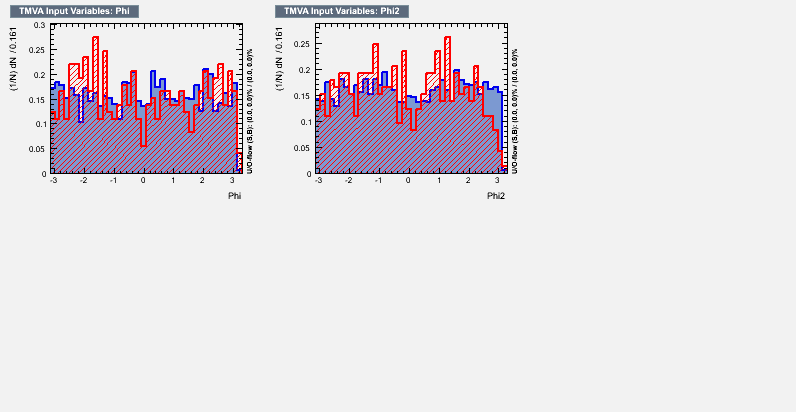
\includegraphics[width=0.8\textwidth]{figs/TMVA_600_nJ2_mu_variables_id_c2.png}	
  \caption{\label{fig:inputs6002jmu}Inputs to the multivariate discriminant for SM Higgs mass of 600~GeV for the 2-jet $W\to\mu\nu$ category}
\end{figure}
%%%%%%%%%%%%%%%%%%%
\newpage
\subsection{Input variables: \texorpdfstring{$M_H$}{M(H)} = 600~GeV, 3 jets}
%%%%%%%%%%%%%%%%%%%
\begin{figure}[ht]
  \centering
  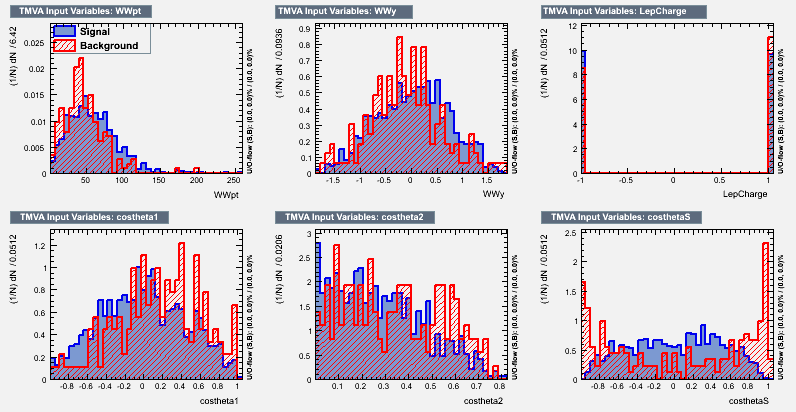
\includegraphics[width=0.8\textwidth]{figs/TMVA_600_nJ3_mu_variables_id_c1.png}
  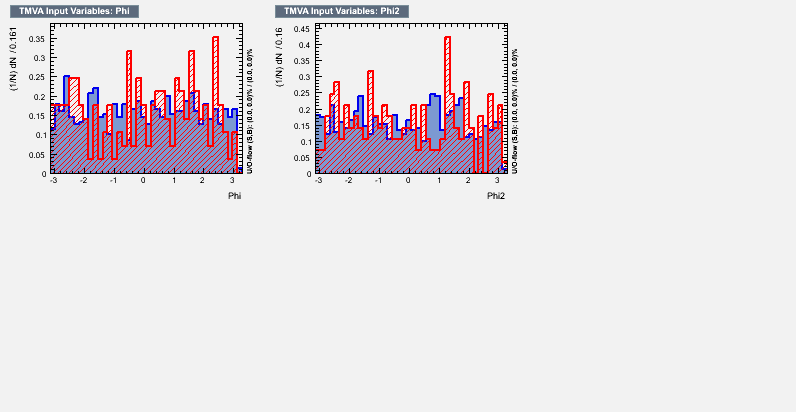
\includegraphics[width=0.8\textwidth]{figs/TMVA_600_nJ3_mu_variables_id_c2.png}	
  \caption{\label{fig:inputs6003jmu}Inputs to the multivariate discriminant for SM Higgs mass of 600~GeV for the 3-jet $W\to\mu\nu$ category}
\end{figure}
%%%%%%%%%%%%%%%%%%%

\newpage
\section{Correlation among the input variables}
Since we use a complete set of minimum number of 
input variables necessary to describe the whole event topology, 
these variables are mostly mostly uncorrelated. 
The correlation matrix for signal and background 
samples are shown in Figs~\ref{fig:FigCorr170Mu}--\ref{fig:FigCorr600Mu}
for various Higgs mass points.
%%%%%%%%%%%%%%%%%%%
\subsection{Correlation matrix: \texorpdfstring{$M_H$}{M(H)} = 170~GeV}
%%%%%%%%%%%%%%%%%%%
\begin{figure}[bthp!]
\subfigure[]{
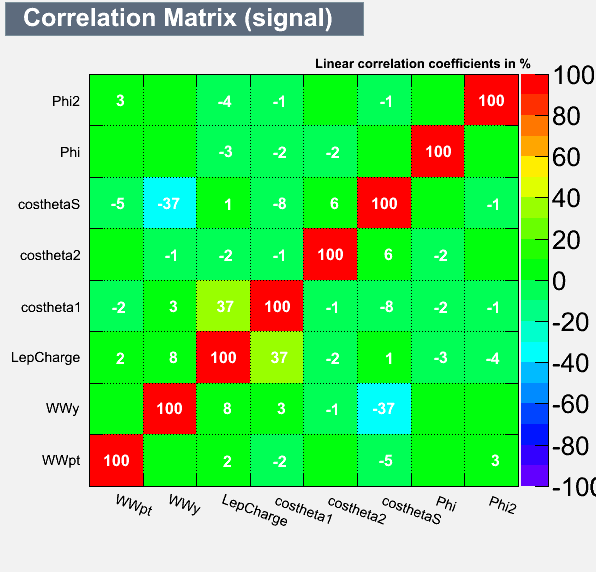
\includegraphics[width=0.49\textwidth]{figs/TMVA_170_nJ2_mu_CorrelationMatrixS}
}
\subfigure[]{
\includegraphics[width=0.49\textwidth]{figs/TMVA_170_nJ2_mu_CorrelationMatrixB}
}
\vspace*{1mm} \\
\subfigure[]{
\includegraphics[width=0.49\textwidth]{figs/TMVA_170_nJ3_mu_CorrelationMatrixS}
}
\subfigure[]{
\includegraphics[width=0.49\textwidth]{figs/TMVA_170_nJ3_mu_CorrelationMatrixB}
}
\caption{\label{fig:FigCorr170Mu} 
Correlation matrix for input variables for Higgs mass point 170 GeV:
(a) signal 2 jets, (b) W+jets background 2 jets, 
(c) signal 3 jets, and (d) W+jets background 3 jets.
}
\end{figure}
%%%%%%%%%%%%%%%%%%%
\newpage
\subsection{Correlation matrix: \texorpdfstring{$M_H$}{M(H)} = 180~GeV}
%%%%%%%%%%%%%%%%%%%
\begin{figure}[bthp!]
\subfigure[]{
\includegraphics[width=0.49\textwidth]{figs/TMVA_180_nJ2_mu_CorrelationMatrixS}
}
\subfigure[]{
\includegraphics[width=0.49\textwidth]{figs/TMVA_180_nJ2_mu_CorrelationMatrixB}
}
\vspace*{1mm} \\
\subfigure[]{
\includegraphics[width=0.49\textwidth]{figs/TMVA_180_nJ3_mu_CorrelationMatrixS}
}
\subfigure[]{
\includegraphics[width=0.49\textwidth]{figs/TMVA_180_nJ3_mu_CorrelationMatrixB}
}
\caption{\label{fig:FigCorr180Mu} 
Correlation matrix for input variables for Higgs mass point 180 GeV:
(a) signal 2 jets, (b) W+jets background 2 jets, 
(c) signal 3 jets, and (d) W+jets background 3 jets.
}
\end{figure}
%%%%%%%%%%%%%%%%%%%
\newpage
\subsection{Correlation matrix: \texorpdfstring{$M_H$}{M(H)} = 190~GeV}
%%%%%%%%%%%%%%%%%%%
\begin{figure}[bthp!]
\subfigure[]{
\includegraphics[width=0.49\textwidth]{figs/TMVA_190_nJ2_mu_CorrelationMatrixS}
}
\subfigure[]{
\includegraphics[width=0.49\textwidth]{figs/TMVA_190_nJ2_mu_CorrelationMatrixB}
}
\vspace*{1mm} \\
\subfigure[]{
\includegraphics[width=0.49\textwidth]{figs/TMVA_190_nJ3_mu_CorrelationMatrixS}
}
\subfigure[]{
\includegraphics[width=0.49\textwidth]{figs/TMVA_190_nJ3_mu_CorrelationMatrixB}
}


\caption{\label{fig:FigCorr190Mu} 
Correlation matrix for input variables for Higgs mass point 190 GeV:
(a) signal 2 jets, (b) W+jets background 2 jets, 
(c) signal 3 jets, and (d) W+jets background 3 jets.
}
\end{figure}
%%%%%%%%%%%%%%%%%%%
\newpage
\subsection{Correlation matrix: \texorpdfstring{$M_H$}{M(H)} = 200~GeV}
%%%%%%%%%%%%%%%%%%%
\begin{figure}[bthp!]
\subfigure[]{
\includegraphics[width=0.49\textwidth]{figs/TMVA_200_nJ2_mu_CorrelationMatrixS}
}
\subfigure[]{
\includegraphics[width=0.49\textwidth]{figs/TMVA_200_nJ2_mu_CorrelationMatrixB}
}
\vspace*{1mm} \\
\subfigure[]{
\includegraphics[width=0.49\textwidth]{figs/TMVA_200_nJ3_mu_CorrelationMatrixS}
}
\subfigure[]{
\includegraphics[width=0.49\textwidth]{figs/TMVA_200_nJ3_mu_CorrelationMatrixB}
}


\caption{\label{fig:FigCorr200Mu} 
Correlation matrix for input variables for Higgs mass point 200 GeV:
(a) signal 2 jets, (b) W+jets background 2 jets, 
(c) signal 3 jets, and (d) W+jets background 3 jets.
}
\end{figure}
%%%%%%%%%%%%%%%%%%%
\newpage
\subsection{Correlation matrix: \texorpdfstring{$M_H$}{M(H)} = 250~GeV}
%%%%%%%%%%%%%%%%%%%
\begin{figure}[bthp!]
\subfigure[]{
\includegraphics[width=0.49\textwidth]{figs/TMVA_250_nJ2_mu_CorrelationMatrixS}
}
\subfigure[]{
\includegraphics[width=0.49\textwidth]{figs/TMVA_250_nJ2_mu_CorrelationMatrixB}
}
\vspace*{1mm} \\
\subfigure[]{
\includegraphics[width=0.49\textwidth]{figs/TMVA_250_nJ3_mu_CorrelationMatrixS}
}
\subfigure[]{
\includegraphics[width=0.49\textwidth]{figs/TMVA_250_nJ3_mu_CorrelationMatrixB}
}


\caption{\label{fig:FigCorr250Mu} 
Correlation matrix for input variables for Higgs mass point 250 GeV:
(a) signal 2 jets, (b) W+jets background 2 jets, 
(c) signal 3 jets, and (d) W+jets background 3 jets.
}
\end{figure}
%%%%%%%%%%%%%%%%%%%
\newpage
\subsection{Correlation matrix: \texorpdfstring{$M_H$}{M(H)} = 300~GeV}
%%%%%%%%%%%%%%%%%%%
\begin{figure}[bthp!]
\subfigure[]{
\includegraphics[width=0.49\textwidth]{figs/TMVA_300_nJ2_mu_CorrelationMatrixS}
}
\subfigure[]{
\includegraphics[width=0.49\textwidth]{figs/TMVA_300_nJ2_mu_CorrelationMatrixB}
}
\vspace*{1mm} \\
\subfigure[]{
\includegraphics[width=0.49\textwidth]{figs/TMVA_300_nJ3_mu_CorrelationMatrixS}
}
\subfigure[]{
\includegraphics[width=0.49\textwidth]{figs/TMVA_300_nJ3_mu_CorrelationMatrixB}
}


\caption{\label{fig:FigCorr300Mu} 
Correlation matrix for input variables for Higgs mass point 300 GeV:
(a) signal 2 jets, (b) W+jets background 2 jets, 
(c) signal 3 jets, and (d) W+jets background 3 jets.
}
\end{figure}
%%%%%%%%%%%%%%%%%%%
\newpage
\subsection{Correlation matrix: \texorpdfstring{$M_H$}{M(H)} = 350~GeV}
%%%%%%%%%%%%%%%%%%%
\begin{figure}[bthp!]
\subfigure[]{
\includegraphics[width=0.49\textwidth]{figs/TMVA_350_nJ2_mu_CorrelationMatrixS}
}
\subfigure[]{
\includegraphics[width=0.49\textwidth]{figs/TMVA_350_nJ2_mu_CorrelationMatrixB}
}
\vspace*{1mm} \\
\subfigure[]{
\includegraphics[width=0.49\textwidth]{figs/TMVA_350_nJ3_mu_CorrelationMatrixS}
}
\subfigure[]{
\includegraphics[width=0.49\textwidth]{figs/TMVA_350_nJ3_mu_CorrelationMatrixB}
}


\caption{\label{fig:FigCorr350Mu} 
Correlation matrix for input variables for Higgs mass point 350 GeV:
(a) signal 2 jets, (b) W+jets background 2 jets, 
(c) signal 3 jets, and (d) W+jets background 3 jets.
}
\end{figure}
%%%%%%%%%%%%%%%%%%%
\newpage
\subsection{Correlation matrix: \texorpdfstring{$M_H$}{M(H)} = 400~GeV}
%%%%%%%%%%%%%%%%%%%
\begin{figure}[bthp!]
\subfigure[]{
\includegraphics[width=0.49\textwidth]{figs/TMVA_400_nJ2_mu_CorrelationMatrixS}
}
\subfigure[]{
\includegraphics[width=0.49\textwidth]{figs/TMVA_400_nJ2_mu_CorrelationMatrixB}
}
\vspace*{1mm} \\
\subfigure[]{
\includegraphics[width=0.49\textwidth]{figs/TMVA_400_nJ3_mu_CorrelationMatrixS}
}
\subfigure[]{
\includegraphics[width=0.49\textwidth]{figs/TMVA_400_nJ3_mu_CorrelationMatrixB}
}


\caption{\label{fig:FigCorr400Mu} 
Correlation matrix for input variables for Higgs mass point 400 GeV:
(a) signal 2 jets, (b) W+jets background 2 jets, 
(c) signal 3 jets, and (d) W+jets background 3 jets.
}
\end{figure}
%%%%%%%%%%%%%%%%%%%
\newpage
\subsection{Correlation matrix: \texorpdfstring{$M_H$}{M(H)} = 450~GeV}
%%%%%%%%%%%%%%%%%%%
\begin{figure}[bthp!]
\subfigure[]{
\includegraphics[width=0.49\textwidth]{figs/TMVA_450_nJ2_mu_CorrelationMatrixS}
}
\subfigure[]{
\includegraphics[width=0.49\textwidth]{figs/TMVA_450_nJ2_mu_CorrelationMatrixB}
}
\vspace*{1mm} \\
\subfigure[]{
\includegraphics[width=0.49\textwidth]{figs/TMVA_450_nJ3_mu_CorrelationMatrixS}
}
\subfigure[]{
\includegraphics[width=0.49\textwidth]{figs/TMVA_450_nJ3_mu_CorrelationMatrixB}
}


\caption{\label{fig:FigCorr450Mu} 
Correlation matrix for input variables for Higgs mass point 450 GeV:
(a) signal 2 jets, (b) W+jets background 2 jets, 
(c) signal 3 jets, and (d) W+jets background 3 jets.
}
\end{figure}
%%%%%%%%%%%%%%%%%%%
\newpage
\subsection{Correlation matrix: \texorpdfstring{$M_H$}{M(H)} = 500~GeV}
%%%%%%%%%%%%%%%%%%%
\begin{figure}[bthp!]
\subfigure[]{
\includegraphics[width=0.49\textwidth]{figs/TMVA_500_nJ2_mu_CorrelationMatrixS}
}
\subfigure[]{
\includegraphics[width=0.49\textwidth]{figs/TMVA_500_nJ2_mu_CorrelationMatrixB}
}
\vspace*{1mm} \\
\subfigure[]{
\includegraphics[width=0.49\textwidth]{figs/TMVA_500_nJ3_mu_CorrelationMatrixS}
}
\subfigure[]{
\includegraphics[width=0.49\textwidth]{figs/TMVA_500_nJ3_mu_CorrelationMatrixB}
}


\caption{\label{fig:FigCorr500Mu} 
Correlation matrix for input variables for Higgs mass point 500 GeV:
(a) signal 2 jets, (b) W+jets background 2 jets, 
(c) signal 3 jets, and (d) W+jets background 3 jets.
}
\end{figure}
%%%%%%%%%%%%%%%%%%%
\newpage
\subsection{Correlation matrix: \texorpdfstring{$M_H$}{M(H)} = 550~GeV}
%%%%%%%%%%%%%%%%%%%
\begin{figure}[bthp!]
\subfigure[]{
\includegraphics[width=0.49\textwidth]{figs/TMVA_550_nJ2_mu_CorrelationMatrixS}
}
\subfigure[]{
\includegraphics[width=0.49\textwidth]{figs/TMVA_550_nJ2_mu_CorrelationMatrixB}
}
\vspace*{1mm} \\
\subfigure[]{
\includegraphics[width=0.49\textwidth]{figs/TMVA_550_nJ3_mu_CorrelationMatrixS}
}
\subfigure[]{
\includegraphics[width=0.49\textwidth]{figs/TMVA_550_nJ3_mu_CorrelationMatrixB}
}


\caption{\label{fig:FigCorr550Mu} 
Correlation matrix for input variables for Higgs mass point 550 GeV:
(a) signal 2 jets, (b) W+jets background 2 jets, 
(c) signal 3 jets, and (d) W+jets background 3 jets.
}
\end{figure}
%%%%%%%%%%%%%%%%%%%
\newpage
\subsection{Correlation matrix: \texorpdfstring{$M_H$}{M(H)} = 600~GeV}
%%%%%%%%%%%%%%%%%%%
\begin{figure}[bthp!]
\subfigure[]{
\includegraphics[width=0.49\textwidth]{figs/TMVA_600_nJ2_mu_CorrelationMatrixS}
}
\subfigure[]{
\includegraphics[width=0.49\textwidth]{figs/TMVA_600_nJ2_mu_CorrelationMatrixB}
}
\vspace*{1mm} \\
\subfigure[]{
\includegraphics[width=0.49\textwidth]{figs/TMVA_600_nJ3_mu_CorrelationMatrixS}
}
\subfigure[]{
\includegraphics[width=0.49\textwidth]{figs/TMVA_600_nJ3_mu_CorrelationMatrixB}
}


\caption{\label{fig:FigCorr600Mu} 
Correlation matrix for input variables for Higgs mass point 600 GeV:
(a) signal 2 jets, (b) W+jets background 2 jets, 
(c) signal 3 jets, and (d) W+jets background 3 jets.
}
\end{figure}
%%%%%%%%%%%%%%%%%%%

\newpage
\section{Output of the MVA training}

The classifier outputs after MVA training for the linear discriminant, 
likelihood, and boosted decision tree 
are shown in Figs~\ref{fig:outputs1702jmu}--\ref{fig:outputs6003jmu}
for various Higgs mass points and jet multiplicities.
%%%%%%%%%%%%%%%%%%%
\subsection{MVA outputs: \texorpdfstring{$M_H$}{M(H)} = 170~GeV, 2 jets}
%%%%%%%%%%%%%%%%%%%
\begin{figure}[ht]
  \centering
  \includegraphics[width=0.32\textwidth]{figs/TMVA_170_nJ2_mu_mva_LD}
  \includegraphics[width=0.32\textwidth]{figs/TMVA_170_nJ2_mu_mva_Likelihood}	
  \includegraphics[width=0.32\textwidth]{figs/TMVA_170_nJ2_mu_mva_BDT}	
  \caption{\label{fig:outputs1702jmu}Output of the multivariate discriminant for SM Higgs mass of 170~GeV for the 2-jet $W\to\mu\nu$ category}
\end{figure}
%%%%%%%%%%%%%%%%%%%
\subsection{MVA outputs: \texorpdfstring{$M_H$}{M(H)} = 170~GeV, 3 jets}
%%%%%%%%%%%%%%%%%%%
\begin{figure}[ht]
  \centering
  \includegraphics[width=0.32\textwidth]{figs/TMVA_170_nJ3_mu_mva_LD}
  \includegraphics[width=0.32\textwidth]{figs/TMVA_170_nJ3_mu_mva_Likelihood}
  \includegraphics[width=0.32\textwidth]{figs/TMVA_170_nJ3_mu_mva_BDT}	
  \caption{\label{fig:outputs1703jmu}Output of the multivariate discriminant for SM Higgs mass of 170~GeV for the 3-jet $W\to\mu\nu$ category}
\end{figure}
%%%%%%%%%%%%%%%%%%%
\subsection{MVA outputs: \texorpdfstring{$M_H$}{M(H)} = 180~GeV, 2 jets}
%%%%%%%%%%%%%%%%%%%
\begin{figure}[ht]
  \centering
  \includegraphics[width=0.32\textwidth]{figs/TMVA_180_nJ2_mu_mva_LD}
  \includegraphics[width=0.32\textwidth]{figs/TMVA_180_nJ2_mu_mva_Likelihood}
  \includegraphics[width=0.32\textwidth]{figs/TMVA_180_nJ2_mu_mva_BDT}	
  \caption{\label{fig:outputs1802jmu}Output of the multivariate discriminant for SM Higgs mass of 180~GeV for the 2-jet $W\to\mu\nu$ category}
\end{figure}
%%%%%%%%%%%%%%%%%%%
\newpage
\subsection{MVA outputs: \texorpdfstring{$M_H$}{M(H)} = 180~GeV, 3 jets}
%%%%%%%%%%%%%%%%%%%
\begin{figure}[ht]
  \centering
  \includegraphics[width=0.32\textwidth]{figs/TMVA_180_nJ3_mu_mva_LD}
  \includegraphics[width=0.32\textwidth]{figs/TMVA_180_nJ3_mu_mva_Likelihood}
  \includegraphics[width=0.32\textwidth]{figs/TMVA_180_nJ3_mu_mva_BDT}	
  \caption{\label{fig:outputs1803jmu}Output of the multivariate discriminant for SM Higgs mass of 180~GeV for the 3-jet $W\to\mu\nu$ category}
\end{figure}
%%%%%%%%%%%%%%%%%%%
\subsection{MVA outputs: \texorpdfstring{$M_H$}{M(H)} = 190~GeV, 2 jets}
%%%%%%%%%%%%%%%%%%%
\begin{figure}[ht]
  \centering
  \includegraphics[width=0.32\textwidth]{figs/TMVA_190_nJ2_mu_mva_LD}
  \includegraphics[width=0.32\textwidth]{figs/TMVA_190_nJ2_mu_mva_Likelihood}
  \includegraphics[width=0.32\textwidth]{figs/TMVA_190_nJ2_mu_mva_BDT}	
  \caption{\label{fig:outputs1902jmu}Output of the multivariate discriminant for SM Higgs mass of 190~GeV for the 2-jet $W\to\mu\nu$ category}
\end{figure}
%%%%%%%%%%%%%%%%%%%
\subsection{MVA outputs: \texorpdfstring{$M_H$}{M(H)} = 190~GeV, 3 jets}
%%%%%%%%%%%%%%%%%%%
\begin{figure}[ht]
  \centering
  \includegraphics[width=0.32\textwidth]{figs/TMVA_190_nJ3_mu_mva_LD}
  \includegraphics[width=0.32\textwidth]{figs/TMVA_190_nJ3_mu_mva_Likelihood}
  \includegraphics[width=0.32\textwidth]{figs/TMVA_190_nJ3_mu_mva_BDT}	
  \caption{\label{fig:outputs1903jmu}Output of the multivariate discriminant for SM Higgs mass of 190~GeV for the 3-jet $W\to\mu\nu$ category}
\end{figure}
%%%%%%%%%%%%%%%%%%%
\newpage
\subsection{MVA outputs: \texorpdfstring{$M_H$}{M(H)} = 200~GeV, 2 jets}
%%%%%%%%%%%%%%%%%%%
\begin{figure}[ht]
  \centering
  \includegraphics[width=0.32\textwidth]{figs/TMVA_200_nJ2_mu_mva_LD}
  \includegraphics[width=0.32\textwidth]{figs/TMVA_200_nJ2_mu_mva_Likelihood}
  \includegraphics[width=0.32\textwidth]{figs/TMVA_200_nJ2_mu_mva_BDT}	
  \caption{\label{fig:outputs2002jmu}Output of the multivariate discriminant for SM Higgs mass of 200~GeV for the 2-jet $W\to\mu\nu$ category}
\end{figure}
%%%%%%%%%%%%%%%%%%%
\subsection{MVA outputs: \texorpdfstring{$M_H$}{M(H)} = 200~GeV, 3 jets}
%%%%%%%%%%%%%%%%%%%
\begin{figure}[ht]
  \centering
  \includegraphics[width=0.32\textwidth]{figs/TMVA_200_nJ3_mu_mva_LD}
  \includegraphics[width=0.32\textwidth]{figs/TMVA_200_nJ3_mu_mva_Likelihood}
  \includegraphics[width=0.32\textwidth]{figs/TMVA_200_nJ3_mu_mva_BDT}	
  \caption{\label{fig:outputs2003jmu}Output of the multivariate discriminant for SM Higgs mass of 200~GeV for the 3-jet $W\to\mu\nu$ category}
\end{figure}
%%%%%%%%%%%%%%%%%%%
\subsection{MVA outputs: \texorpdfstring{$M_H$}{M(H)} = 250~GeV, 2 jets}
%%%%%%%%%%%%%%%%%%%
\begin{figure}[ht]
  \centering
  \includegraphics[width=0.32\textwidth]{figs/TMVA_250_nJ2_mu_mva_LD}
  \includegraphics[width=0.32\textwidth]{figs/TMVA_250_nJ2_mu_mva_Likelihood}
  \includegraphics[width=0.32\textwidth]{figs/TMVA_250_nJ2_mu_mva_BDT}	
  \caption{\label{fig:outputs2502jmu}Output of the multivariate discriminant for SM Higgs mass of 250~GeV for the 2-jet $W\to\mu\nu$ category}
\end{figure}
%%%%%%%%%%%%%%%%%%%
\newpage
\subsection{MVA outputs: \texorpdfstring{$M_H$}{M(H)} = 250~GeV, 3 jets}
%%%%%%%%%%%%%%%%%%%
\begin{figure}[ht]
  \centering
  \includegraphics[width=0.32\textwidth]{figs/TMVA_250_nJ3_mu_mva_LD}
  \includegraphics[width=0.32\textwidth]{figs/TMVA_250_nJ3_mu_mva_Likelihood}
  \includegraphics[width=0.32\textwidth]{figs/TMVA_250_nJ3_mu_mva_BDT}
  \caption{\label{fig:outputs2503jmu}Output of the multivariate discriminant for SM Higgs mass of 250~GeV for the 3-jet $W\to\mu\nu$ category}
\end{figure}
%%%%%%%%%%%%%%%%%%%
\subsection{MVA outputs: \texorpdfstring{$M_H$}{M(H)} = 300~GeV, 2 jets}
%%%%%%%%%%%%%%%%%%%
\begin{figure}[ht]
  \centering
  \includegraphics[width=0.32\textwidth]{figs/TMVA_300_nJ2_mu_mva_LD}
  \includegraphics[width=0.32\textwidth]{figs/TMVA_300_nJ2_mu_mva_Likelihood}
  \includegraphics[width=0.32\textwidth]{figs/TMVA_300_nJ2_mu_mva_BDT}	
  \caption{\label{fig:outputs3002jmu}Output of the multivariate discriminant for SM Higgs mass of 300~GeV for the 2-jet $W\to\mu\nu$ category}
\end{figure}
%%%%%%%%%%%%%%%%%%%
\subsection{MVA outputs: \texorpdfstring{$M_H$}{M(H)} = 300~GeV, 3 jets}
%%%%%%%%%%%%%%%%%%%
\begin{figure}[ht]
  \centering
  \includegraphics[width=0.32\textwidth]{figs/TMVA_300_nJ3_mu_mva_LD}
  \includegraphics[width=0.32\textwidth]{figs/TMVA_300_nJ3_mu_mva_Likelihood}	
  \includegraphics[width=0.32\textwidth]{figs/TMVA_300_nJ3_mu_mva_BDT}
  \caption{\label{fig:outputs3003jmu}Output of the multivariate discriminant for SM Higgs mass of 300~GeV for the 3-jet $W\to\mu\nu$ category}
\end{figure}
%%%%%%%%%%%%%%%%%%%
\newpage
\subsection{MVA outputs: \texorpdfstring{$M_H$}{M(H)} = 350~GeV, 2 jets}
%%%%%%%%%%%%%%%%%%%
\begin{figure}[ht]
  \centering
  \includegraphics[width=0.32\textwidth]{figs/TMVA_350_nJ2_mu_mva_LD}
  \includegraphics[width=0.32\textwidth]{figs/TMVA_350_nJ2_mu_mva_Likelihood}
  \includegraphics[width=0.32\textwidth]{figs/TMVA_350_nJ2_mu_mva_BDT}	
  \caption{\label{fig:outputs3502jmu}Output of the multivariate discriminant for SM Higgs mass of 350~GeV for the 2-jet $W\to\mu\nu$ category}
\end{figure}
%%%%%%%%%%%%%%%%%%%
\subsection{MVA outputs: \texorpdfstring{$M_H$}{M(H)} = 350~GeV, 3 jets}
%%%%%%%%%%%%%%%%%%%
\begin{figure}[ht]
  \centering
  \includegraphics[width=0.32\textwidth]{figs/TMVA_350_nJ3_mu_mva_LD}
  \includegraphics[width=0.32\textwidth]{figs/TMVA_350_nJ3_mu_mva_Likelihood}
  \includegraphics[width=0.32\textwidth]{figs/TMVA_350_nJ3_mu_mva_BDT}	
  \caption{\label{fig:outputs3503jmu}Output of the multivariate discriminant for SM Higgs mass of 350~GeV for the 3-jet $W\to\mu\nu$ category}
\end{figure}
%%%%%%%%%%%%%%%%%%%
\subsection{MVA outputs: \texorpdfstring{$M_H$}{M(H)} = 400~GeV, 2 jets}
%%%%%%%%%%%%%%%%%%%
\begin{figure}[ht]
  \centering
  \includegraphics[width=0.32\textwidth]{figs/TMVA_400_nJ2_mu_mva_LD}
  \includegraphics[width=0.32\textwidth]{figs/TMVA_400_nJ2_mu_mva_Likelihood}
  \includegraphics[width=0.32\textwidth]{figs/TMVA_400_nJ2_mu_mva_BDT}	
  \caption{\label{fig:outputs4002jmu}Output of the multivariate discriminant for SM Higgs mass of 400~GeV for the 2-jet $W\to\mu\nu$ category}
\end{figure}
%%%%%%%%%%%%%%%%%%%
\newpage
\subsection{MVA outputs: \texorpdfstring{$M_H$}{M(H)} = 400~GeV, 3 jets}
%%%%%%%%%%%%%%%%%%%
\begin{figure}[ht]
  \centering
  \includegraphics[width=0.32\textwidth]{figs/TMVA_400_nJ3_mu_mva_LD}
  \includegraphics[width=0.32\textwidth]{figs/TMVA_400_nJ3_mu_mva_Likelihood}
  \includegraphics[width=0.32\textwidth]{figs/TMVA_400_nJ3_mu_mva_BDT}	
  \caption{\label{fig:outputs4003jmu}Output of the multivariate discriminant for SM Higgs mass of 400~GeV for the 3-jet $W\to\mu\nu$ category}
\end{figure}
%%%%%%%%%%%%%%%%%%%
\subsection{MVA outputs: \texorpdfstring{$M_H$}{M(H)} = 450~GeV, 2 jets}
%%%%%%%%%%%%%%%%%%%
\begin{figure}[ht]
  \centering
  \includegraphics[width=0.32\textwidth]{figs/TMVA_450_nJ2_mu_mva_LD}
  \includegraphics[width=0.32\textwidth]{figs/TMVA_450_nJ2_mu_mva_Likelihood}
  \includegraphics[width=0.32\textwidth]{figs/TMVA_450_nJ2_mu_mva_BDT}	
  \caption{\label{fig:outputs4502jmu}Output of the multivariate discriminant for SM Higgs mass of 450~GeV for the 2-jet $W\to\mu\nu$ category}
\end{figure}
%%%%%%%%%%%%%%%%%%%
\subsection{MVA outputs: \texorpdfstring{$M_H$}{M(H)} = 450~GeV, 3 jets}
%%%%%%%%%%%%%%%%%%%
\begin{figure}[ht]
  \centering
  \includegraphics[width=0.32\textwidth]{figs/TMVA_450_nJ3_mu_mva_LD}
  \includegraphics[width=0.32\textwidth]{figs/TMVA_450_nJ3_mu_mva_Likelihood}
  \includegraphics[width=0.32\textwidth]{figs/TMVA_450_nJ3_mu_mva_BDT}	
  \caption{\label{fig:outputs4503jmu}Output of the multivariate discriminant for SM Higgs mass of 450~GeV for the 3-jet $W\to\mu\nu$ category}
\end{figure}
%%%%%%%%%%%%%%%%%%%
\newpage
\subsection{MVA outputs: \texorpdfstring{$M_H$}{M(H)} = 500~GeV, 2 jets}
%%%%%%%%%%%%%%%%%%%
\begin{figure}[ht]
  \centering
  \includegraphics[width=0.32\textwidth]{figs/TMVA_500_nJ2_mu_mva_LD}
  \includegraphics[width=0.32\textwidth]{figs/TMVA_500_nJ2_mu_mva_Likelihood}
  \includegraphics[width=0.32\textwidth]{figs/TMVA_500_nJ2_mu_mva_BDT}	
  \caption{\label{fig:outputs5002jmu}Output of the multivariate discriminant for SM Higgs mass of 500~GeV for the 2-jet $W\to\mu\nu$ category}
\end{figure}
%%%%%%%%%%%%%%%%%%%
\subsection{MVA outputs: \texorpdfstring{$M_H$}{M(H)} = 500~GeV, 3 jets}
%%%%%%%%%%%%%%%%%%%
\begin{figure}[ht]
  \centering
  \includegraphics[width=0.32\textwidth]{figs/TMVA_500_nJ3_mu_mva_LD}
  \includegraphics[width=0.32\textwidth]{figs/TMVA_500_nJ3_mu_mva_Likelihood}
  \includegraphics[width=0.32\textwidth]{figs/TMVA_500_nJ3_mu_mva_BDT}	
  \caption{\label{fig:outputs5003jmu}Output of the multivariate discriminant for SM Higgs mass of 500~GeV for the 3-jet $W\to\mu\nu$ category}
\end{figure}
%%%%%%%%%%%%%%%%%%%
\subsection{MVA outputs: \texorpdfstring{$M_H$}{M(H)} = 550~GeV, 2 jets}
%%%%%%%%%%%%%%%%%%%
\begin{figure}[ht]
  \centering
  \includegraphics[width=0.32\textwidth]{figs/TMVA_550_nJ2_mu_mva_LD}
  \includegraphics[width=0.32\textwidth]{figs/TMVA_550_nJ2_mu_mva_Likelihood}
  \includegraphics[width=0.32\textwidth]{figs/TMVA_550_nJ2_mu_mva_BDT}	
  \caption{\label{fig:outputs5502jmu}Output of the multivariate discriminant for SM Higgs mass of 550~GeV for the 2-jet $W\to\mu\nu$ category}
\end{figure}
%%%%%%%%%%%%%%%%%%%
\newpage
\subsection{MVA outputs: \texorpdfstring{$M_H$}{M(H)} = 550~GeV, 3 jets}
%%%%%%%%%%%%%%%%%%%
\begin{figure}[ht]
  \centering
  \includegraphics[width=0.32\textwidth]{figs/TMVA_550_nJ3_mu_mva_LD}
  \includegraphics[width=0.32\textwidth]{figs/TMVA_550_nJ3_mu_mva_Likelihood}
  \includegraphics[width=0.32\textwidth]{figs/TMVA_550_nJ3_mu_mva_BDT}	
  \caption{\label{fig:outputs5503jmu}Output of the multivariate discriminant for SM Higgs mass of 550~GeV for the 3-jet $W\to\mu\nu$ category}
\end{figure}
%%%%%%%%%%%%%%%%%%%
\subsection{MVA outputs: \texorpdfstring{$M_H$}{M(H)} = 600~GeV, 2 jets}
%%%%%%%%%%%%%%%%%%%
\begin{figure}[ht]
  \centering
  \includegraphics[width=0.32\textwidth]{figs/TMVA_600_nJ2_mu_mva_LD}
  \includegraphics[width=0.32\textwidth]{figs/TMVA_600_nJ2_mu_mva_Likelihood}
  \includegraphics[width=0.32\textwidth]{figs/TMVA_600_nJ2_mu_mva_BDT}	
  \caption{\label{fig:outputs6002jmu}Output of the multivariate discriminant for SM Higgs mass of 600~GeV for the 2-jet $W\to\mu\nu$ category}
\end{figure}
%%%%%%%%%%%%%%%%%%%
\subsection{MVA outputs: \texorpdfstring{$M_H$}{M(H)} = 600~GeV, 3 jets}
%%%%%%%%%%%%%%%%%%%
\begin{figure}[ht]
  \centering
  \includegraphics[width=0.32\textwidth]{figs/TMVA_600_nJ3_mu_mva_LD}
  \includegraphics[width=0.32\textwidth]{figs/TMVA_600_nJ3_mu_mva_Likelihood}
  \includegraphics[width=0.32\textwidth]{figs/TMVA_600_nJ3_mu_mva_BDT}	
  \caption{\label{fig:outputs6003jmu}Output of the multivariate discriminant for SM Higgs mass of 600~GeV for the 3-jet $W\to\mu\nu$ category}
\end{figure}
%%%%%%%%%%%%%%%%%%%

\newpage
\section{Performance: signal efficiency vs. background rejection rate}

The performance of the three classifiers -- linear discriminant, 
likelihood, and boosted decision tree -- 
are shown in Figs~\ref{fig:perf170mu}--\ref{fig:perf600mu}
for various Higgs mass points in terms of signal efficiency versus background rejection rate 
as the figure of merit.
The likelihood gives the best discrimination, therefore we use it 
for our analysis as will be described in detail in the next section.
%%%%%%%%%%%%%%%%%%%
\subsection{MVA performance: \texorpdfstring{$M_H$}{M(H)} = 170~GeV}
%%%%%%%%%%%%%%%%%%%
\begin{figure}[ht]
  \centering
  \includegraphics[width=0.48\textwidth]{figs/TMVA_170_nJ2_mu_rejBvsS}
  \includegraphics[width=0.48\textwidth]{figs/TMVA_170_nJ3_mu_rejBvsS}	
  \caption{\label{fig:perf170mu}Inputs to the multivariate discriminant for SM Higgs mass of 170~GeV for (a) 2-jet and (b) 3-jet $W\to\mu\nu$ category}
\end{figure}
%%%%%%%%%%%%%%%%%%%
\subsection{MVA performance: \texorpdfstring{$M_H$}{M(H)} = 180~GeV}
%%%%%%%%%%%%%%%%%%%
\begin{figure}[ht]
  \centering
  \includegraphics[width=0.48\textwidth]{figs/TMVA_180_nJ2_mu_rejBvsS}
  \includegraphics[width=0.48\textwidth]{figs/TMVA_180_nJ3_mu_rejBvsS}	
  \caption{\label{fig:perf180mu}Inputs to the multivariate discriminant for SM Higgs mass of 180~GeV for (a) 2-jet and (b) 3-jet $W\to\mu\nu$ category}
\end{figure}
%%%%%%%%%%%%%%%%%%%
\newpage
\subsection{MVA performance: \texorpdfstring{$M_H$}{M(H)} = 190~GeV}
%%%%%%%%%%%%%%%%%%%
\begin{figure}[ht]
  \centering
  \includegraphics[width=0.48\textwidth]{figs/TMVA_190_nJ2_mu_rejBvsS}
  \includegraphics[width=0.48\textwidth]{figs/TMVA_190_nJ3_mu_rejBvsS}	
  \caption{\label{fig:perf190mu}Inputs to the multivariate discriminant for SM Higgs mass of 190~GeV for (a) 2-jet and (b) 3-jet $W\to\mu\nu$ category}
\end{figure}
%%%%%%%%%%%%%%%%%%%
\subsection{MVA performance: \texorpdfstring{$M_H$}{M(H)} = 200~GeV}
%%%%%%%%%%%%%%%%%%%
\begin{figure}[ht]
  \centering
  \includegraphics[width=0.48\textwidth]{figs/TMVA_200_nJ2_mu_rejBvsS}
  \includegraphics[width=0.48\textwidth]{figs/TMVA_200_nJ3_mu_rejBvsS}	
  \caption{\label{fig:perf200mu}Inputs to the multivariate discriminant for SM Higgs mass of 200~GeV for (a) 2-jet and (b) 3-jet $W\to\mu\nu$ category}
\end{figure}
%%%%%%%%%%%%%%%%%%%
\newpage
\subsection{MVA performance: \texorpdfstring{$M_H$}{M(H)} = 250~GeV}
%%%%%%%%%%%%%%%%%%%
\begin{figure}[ht]
  \centering
  \includegraphics[width=0.48\textwidth]{figs/TMVA_250_nJ2_mu_rejBvsS}
  \includegraphics[width=0.48\textwidth]{figs/TMVA_250_nJ3_mu_rejBvsS}	
  \caption{\label{fig:perf250mu}Inputs to the multivariate discriminant for SM Higgs mass of 250~GeV for (a) 2-jet and (b) 3-jet $W\to\mu\nu$ category}
\end{figure}
%%%%%%%%%%%%%%%%%%%
\subsection{MVA performance: \texorpdfstring{$M_H$}{M(H)} = 300~GeV}
%%%%%%%%%%%%%%%%%%%
\begin{figure}[ht]
  \centering
  \includegraphics[width=0.48\textwidth]{figs/TMVA_300_nJ2_mu_rejBvsS}
  \includegraphics[width=0.48\textwidth]{figs/TMVA_300_nJ3_mu_rejBvsS}	
  \caption{\label{fig:perf300mu}Inputs to the multivariate discriminant for SM Higgs mass of 300~GeV for (a) 2-jet and (b) 3-jet $W\to\mu\nu$ category}
\end{figure}
%%%%%%%%%%%%%%%%%%%
\newpage
\subsection{MVA performance: \texorpdfstring{$M_H$}{M(H)} = 350~GeV}
%%%%%%%%%%%%%%%%%%%
\begin{figure}[ht]
  \centering
  \includegraphics[width=0.48\textwidth]{figs/TMVA_350_nJ2_mu_rejBvsS}
  \includegraphics[width=0.48\textwidth]{figs/TMVA_350_nJ3_mu_rejBvsS}	
  \caption{\label{fig:perf350mu}Inputs to the multivariate discriminant for SM Higgs mass of 350~GeV for (a) 2-jet and (b) 3-jet $W\to\mu\nu$ category}
\end{figure}
%%%%%%%%%%%%%%%%%%%
\subsection{MVA performance: \texorpdfstring{$M_H$}{M(H)} = 400~GeV}
%%%%%%%%%%%%%%%%%%%
\begin{figure}[ht]
  \centering
  \includegraphics[width=0.48\textwidth]{figs/TMVA_400_nJ2_mu_rejBvsS}
  \includegraphics[width=0.48\textwidth]{figs/TMVA_400_nJ3_mu_rejBvsS}	
  \caption{\label{fig:perf400mu}Inputs to the multivariate discriminant for SM Higgs mass of 400~GeV for (a) 2-jet and (b) 3-jet $W\to\mu\nu$ category}
\end{figure}
%%%%%%%%%%%%%%%%%%%
\newpage
\subsection{MVA performance: \texorpdfstring{$M_H$}{M(H)} = 450~GeV}
%%%%%%%%%%%%%%%%%%%
\begin{figure}[ht]
  \centering
  \includegraphics[width=0.48\textwidth]{figs/TMVA_450_nJ2_mu_rejBvsS}
  \includegraphics[width=0.48\textwidth]{figs/TMVA_450_nJ3_mu_rejBvsS}	
  \caption{\label{fig:perf450mu}Inputs to the multivariate discriminant for SM Higgs mass of 450~GeV for (a) 2-jet and (b) 3-jet $W\to\mu\nu$ category}
\end{figure}
%%%%%%%%%%%%%%%%%%%
\subsection{MVA performance: \texorpdfstring{$M_H$}{M(H)} = 500~GeV}
%%%%%%%%%%%%%%%%%%%
\begin{figure}[ht]
  \centering
  \includegraphics[width=0.48\textwidth]{figs/TMVA_500_nJ2_mu_rejBvsS}
  \includegraphics[width=0.48\textwidth]{figs/TMVA_500_nJ3_mu_rejBvsS}	
  \caption{\label{fig:perf500mu}Inputs to the multivariate discriminant for SM Higgs mass of 500~GeV for (a) 2-jet and (b) 3-jet $W\to\mu\nu$ category}
\end{figure}
%%%%%%%%%%%%%%%%%%%
\newpage
\subsection{MVA performance: \texorpdfstring{$M_H$}{M(H)} = 550~GeV}
%%%%%%%%%%%%%%%%%%%
\begin{figure}[ht]
  \centering
  \includegraphics[width=0.48\textwidth]{figs/TMVA_550_nJ2_mu_rejBvsS}
  \includegraphics[width=0.48\textwidth]{figs/TMVA_550_nJ3_mu_rejBvsS}	
  \caption{\label{fig:perf550mu}Inputs to the multivariate discriminant for SM Higgs mass of 550~GeV for (a) 2-jet and (b) 3-jet $W\to\mu\nu$ category}
\end{figure}
%%%%%%%%%%%%%%%%%%%
\subsection{MVA performance: \texorpdfstring{$M_H$}{M(H)} = 600~GeV}
%%%%%%%%%%%%%%%%%%%
\begin{figure}[ht]
  \centering
  \includegraphics[width=0.48\textwidth]{figs/TMVA_600_nJ2_mu_rejBvsS}
  \includegraphics[width=0.48\textwidth]{figs/TMVA_600_nJ3_mu_rejBvsS}	
  \caption{\label{fig:perf600mu}Inputs to the multivariate discriminant for SM Higgs mass of 600~GeV for (a) 2-jet and (b) 3-jet $W\to\mu\nu$ category}
\end{figure}
%%%%%%%%%%%%%%%%%%%

\newpage
\section{Ranking of the input variables}
Below we print out the ranking of
the input variables in order of their discriminating power.
In summary:
%%%%%%%%%%%%%%%%
\begin{itemize}
\item  The consistent picture among all the mass points is that the 
quark-gluon likelihoods are always quite high in the ranking.
\item  The variable rankings depend strongly on mH and to somewhat
   on nJets.
   \begin{itemize}
   \item  For High Higgs mass (let's say, $m_H > 250$ GeV), $\cos\theta^*$
        is generally ranked 1, followed by  the two quark-gluon
        likelihoods, and $\cos\theta_2$.
    \item  For low Higgs mass points ($< 250$ GeV) the exact ordering of the
        variables changes by mass point, but the most discriminating
        ones are lepton charge, QG likelihoods, $\cos\theta{1,2}$, 
        and $\cos\theta^*$.
     \end{itemize}

\item  At times, some variable contributes negatively (although not hugely)
to the likelihood. In principle, one can improve the performance of
likelihood for a few mH points by removing such a variable from the
input list.
\end{itemize}
%%%%%%%%%%%%%%%%


%%\begin{verbatim}
%%=============================
%%mH = 170 GeV, nJets = 2
%%=============================
%% ----------------------------------------
%% Rank : Variable  : Delta Separation
%% ----------------------------------------
%%    1 : LepCharge : 2.034e-02
%%    2 : J2QGL     : 1.690e-02
%%    3 : costheta2 : 1.264e-02
%%    4 : J1QGL     : 8.168e-03
%%    5 : costheta1 : 7.571e-03
%%    6 : Phi       : 7.017e-03
%%    7 : WWy       : 4.226e-03
%%    8 : costhetaS : 2.466e-03
%%    9 : Phi2      : 4.410e-04
%%   10 : WWpt      : -5.390e-04
%% ----------------------------------------
%%
%%=============================
%%mH = 170 GeV, nJets = 3
%%=============================
%% ----------------------------------------
%% Rank : Variable  : Delta Separation
%% ----------------------------------------
%%    1 : LepCharge : 3.317e-02
%%    2 : WWy       : 2.391e-02
%%    3 : J1QGL     : 2.269e-02
%%    4 : J2QGL     : 1.306e-02
%%    5 : costheta2 : 7.705e-03
%%    6 : costheta1 : 6.121e-03
%%    7 : WWpt      : 2.428e-03
%%    8 : Phi       : 1.777e-03
%%    9 : costhetaS : -6.589e-03
%%   10 : Phi2      : -2.014e-02
%% ----------------------------------------
%%
%%=============================
%%mH = 180 GeV, nJets = 2
%%=============================
%% ----------------------------------------
%% Rank : Variable  : Delta Separation
%% ----------------------------------------
%%    1 : costhetaS : 3.265e-02
%%    2 : J2QGL     : 2.068e-02
%%    3 : J1QGL     : 1.767e-02
%%    4 : Phi2      : 1.683e-02
%%    5 : LepCharge : 1.093e-02
%%    6 : costheta2 : 8.688e-03
%%    7 : costheta1 : 7.388e-03
%%    8 : WWy       : 6.885e-03
%%    9 : Phi       : 5.061e-03
%%   10 : WWpt      : 3.488e-03
%% ----------------------------------------
%%
%%=============================
%%mH = 180 GeV, nJets = 3
%%=============================
%% ----------------------------------------
%% Rank : Variable  : Delta Separation
%% ----------------------------------------
%%    1 : J2QGL     : 5.089e-03
%%    2 : WWpt      : 1.609e-03
%%    3 : J1QGL     : 4.806e-05
%%    4 : costhetaS : -4.665e-04
%%    5 : Phi2      : -6.580e-03
%%    6 : WWy       : -7.403e-03
%%    7 : LepCharge : -8.175e-03
%%    8 : costheta1 : -9.772e-03
%%    9 : costheta2 : -1.844e-02
%%   10 : Phi       : -2.465e-02
%% ----------------------------------------
%%
%%=============================
%%mH = 190 GeV, nJets = 2
%%=============================
%% ----------------------------------------
%% Rank : Variable  : Delta Separation
%% ----------------------------------------
%%    1 : costhetaS : 6.676e-02
%%    2 : Phi2      : 1.767e-02
%%    3 : J2QGL     : 1.321e-02
%%    4 : costheta1 : 4.538e-03
%%    5 : J1QGL     : 1.017e-03
%%    6 : WWy       : 9.787e-04
%%    7 : LepCharge : 5.541e-04
%%    8 : WWpt      : -1.202e-03
%%    9 : costheta2 : -2.097e-03
%%   10 : Phi       : -2.679e-03
%% ----------------------------------------
%%
%%=============================
%%mH = 190 GeV, nJets = 3
%%=============================
%% ----------------------------------------
%% Rank : Variable  : Delta Separation
%% ----------------------------------------
%%    1 : J2QGL     : 3.582e-02
%%    2 : costheta1 : 2.572e-02
%%    3 : J1QGL     : 1.991e-02
%%    4 : Phi       : 1.906e-02
%%    5 : costhetaS : 1.706e-02
%%    6 : LepCharge : 1.520e-02
%%    7 : Phi2      : 1.241e-02
%%    8 : WWpt      : 1.021e-02
%%    9 : costheta2 : 1.648e-03
%%   10 : WWy       : 1.058e-04
%% ----------------------------------------
%%
%%=============================
%%mH = 200 GeV, nJets = 2
%%=============================
%% ----------------------------------------
%% Rank : Variable  : Delta Separation
%% ----------------------------------------
%%    1 : costhetaS : 1.059e-01
%%    2 : J2QGL     : 3.846e-02
%%    3 : Phi2      : 2.053e-02
%%    4 : J1QGL     : 9.455e-03
%%    5 : Phi       : 8.157e-03
%%    6 : LepCharge : 6.910e-03
%%    7 : costheta2 : 5.306e-03
%%    8 : WWy       : 4.508e-03
%%    9 : costheta1 : 3.725e-03
%%   10 : WWpt      : 1.751e-03
%% ----------------------------------------
%%
%%=============================
%%mH = 200 GeV, nJets = 3
%%=============================
%% ----------------------------------------
%% Rank : Variable  : Delta Separation
%% ----------------------------------------
%%    1 : costhetaS : 6.229e-02
%%    2 : Phi2      : 1.097e-02
%%    3 : LepCharge : 9.042e-03
%%    4 : WWpt      : 5.278e-03
%%    5 : costheta2 : -1.482e-03
%%    6 : Phi       : -5.930e-03
%%    7 : costheta1 : -9.963e-03
%%    8 : J2QGL     : -1.225e-02
%%    9 : WWy       : -1.591e-02
%%   10 : J1QGL     : -1.682e-02
%% ----------------------------------------
%%
%%=============================
%%mH = 250 GeV, nJets = 2
%%=============================
%% ----------------------------------------
%% Rank : Variable  : Delta Separation
%% ----------------------------------------
%%    1 : costhetaS : 1.977e-01
%%    2 : J2QGL     : 1.879e-02
%%    3 : costheta2 : 1.019e-02
%%    4 : Phi2      : 8.876e-03
%%    5 : costheta1 : 4.892e-03
%%    6 : J1QGL     : 4.373e-03
%%    7 : WWpt      : 3.091e-03
%%    8 : LepCharge : 1.860e-03
%%    9 : Phi       : -8.182e-04
%%   10 : WWy       : -8.728e-03
%% ----------------------------------------
%%
%%=============================
%%mH = 250 GeV, nJets = 3
%%=============================
%% ----------------------------------------
%% Rank : Variable  : Delta Separation
%% ----------------------------------------
%%    1 : costhetaS : 1.443e-01
%%    2 : WWy       : 1.361e-02
%%    3 : costheta1 : 1.250e-02
%%    4 : LepCharge : 1.193e-02
%%    5 : J2QGL     : 1.138e-02
%%    6 : J1QGL     : 9.706e-03
%%    7 : Phi2      : 8.026e-03
%%    8 : costheta2 : 6.031e-03
%%    9 : WWpt      : 4.446e-03
%%   10 : Phi       : 2.781e-03
%% ----------------------------------------
%%
%%=============================
%%mH = 300 GeV, nJets = 2
%%=============================
%% ----------------------------------------
%% Rank : Variable  : Delta Separation
%% ----------------------------------------
%%    1 : costhetaS : 2.401e-01
%%    2 : J2QGL     : 2.465e-02
%%    3 : costheta2 : 1.389e-02
%%    4 : costheta1 : 1.270e-02
%%    5 : LepCharge : 6.117e-03
%%    6 : Phi       : 5.590e-03
%%    7 : Phi2      : 5.568e-03
%%    8 : J1QGL     : 4.795e-03
%%    9 : WWpt      : 4.712e-03
%%   10 : WWy       : -8.953e-03
%% ----------------------------------------
%%
%%=============================
%%mH = 300 GeV, nJets = 3
%%=============================
%% ----------------------------------------
%% Rank : Variable  : Delta Separation
%% ----------------------------------------
%%    1 : costhetaS : 1.639e-01
%%    2 : J2QGL     : 2.213e-02
%%    3 : costheta1 : 2.050e-02
%%    4 : Phi2      : 7.890e-03
%%    5 : costheta2 : 7.000e-03
%%    6 : WWpt      : 6.566e-03
%%    7 : LepCharge : 4.602e-03
%%    8 : J1QGL     : 3.248e-03
%%    9 : WWy       : 1.120e-04
%%   10 : Phi       : -9.648e-03
%% ----------------------------------------
%%
%%=============================
%%mH = 350 GeV, nJets = 2
%%=============================
%% ----------------------------------------
%% Rank : Variable  : Delta Separation
%% ----------------------------------------
%%    1 : costhetaS : 2.477e-01
%%    2 : costheta2 : 2.187e-02
%%    3 : J2QGL     : 1.227e-02
%%    4 : LepCharge : 6.979e-03
%%    5 : costheta1 : 6.972e-03
%%    6 : Phi2      : 3.565e-03
%%    7 : WWpt      : 2.977e-03
%%    8 : J1QGL     : 2.382e-03
%%    9 : Phi       : 1.925e-03
%%   10 : WWy       : -1.712e-02
%% ----------------------------------------
%%
%%=============================
%%mH = 350 GeV, nJets = 3
%%=============================
%% ----------------------------------------
%% Rank : Variable  : Delta Separation
%% ----------------------------------------
%%    1 : costhetaS : 2.090e-01
%%    2 : costheta2 : 2.041e-02
%%    3 : J2QGL     : 1.584e-02
%%    4 : Phi2      : 1.495e-02
%%    5 : J1QGL     : 1.223e-02
%%    6 : costheta1 : 1.181e-02
%%    7 : WWpt      : 1.022e-02
%%    8 : LepCharge : 4.994e-03
%%    9 : Phi       : 4.533e-03
%%   10 : WWy       : 2.997e-03
%% ----------------------------------------
%%
%%=============================
%%mH = 400 GeV, nJets = 2
%%=============================
%% ----------------------------------------
%% Rank : Variable  : Delta Separation
%% ----------------------------------------
%%    1 : costhetaS : 2.259e-01
%%    2 : J2QGL     : 1.605e-02
%%    3 : costheta2 : 1.444e-02
%%    4 : LepCharge : 4.634e-03
%%    5 : J1QGL     : 3.558e-03
%%    6 : WWpt      : 8.403e-04
%%    7 : Phi       : -8.863e-04
%%    8 : Phi2      : -1.124e-03
%%    9 : costheta1 : -1.136e-03
%%   10 : WWy       : -2.392e-02
%% ----------------------------------------
%%
%%=============================
%%mH = 400 GeV, nJets = 3
%%=============================
%% ----------------------------------------
%% Rank : Variable  : Delta Separation
%% ----------------------------------------
%%    1 : costhetaS : 2.015e-01
%%    2 : costheta1 : 4.996e-02
%%    3 : J2QGL     : 4.883e-02
%%    4 : LepCharge : 3.327e-02
%%    5 : WWy       : 3.272e-02
%%    6 : WWpt      : 3.011e-02
%%    7 : costheta2 : 2.689e-02
%%    8 : Phi2      : 2.160e-02
%%    9 : Phi       : 1.601e-02
%%   10 : J1QGL     : 1.109e-02
%% ----------------------------------------
%%
%%=============================
%%450 GeV, nJets = 2
%%=============================
%% ----------------------------------------
%% Rank : Variable  : Delta Separation
%% ----------------------------------------
%%    1 : costhetaS : 2.299e-01
%%    2 : costheta2 : 2.091e-02
%%    3 : J1QGL     : 1.849e-02
%%    4 : J2QGL     : 1.713e-02
%%    5 : costheta1 : 9.618e-03
%%    6 : Phi2      : 9.437e-03
%%    7 : LepCharge : 5.517e-03
%%    8 : WWpt      : 5.053e-03
%%    9 : Phi       : -1.532e-03
%%   10 : WWy       : -1.415e-02
%% ----------------------------------------
%%
%%=============================
%%mH = 450 GeV, nJets = 3
%%=============================
%% ----------------------------------------
%% Rank : Variable  : Delta Separation
%% ----------------------------------------
%%    1 : costhetaS : 1.818e-01
%%    2 : J2QGL     : 4.135e-02
%%    3 : costheta1 : 9.994e-03
%%    4 : LepCharge : 6.463e-03
%%    5 : WWy       : 1.677e-03
%%    6 : J1QGL     : -2.145e-03
%%    7 : WWpt      : -3.273e-03
%%    8 : costheta2 : -4.418e-03
%%    9 : Phi       : -8.651e-03
%%   10 : Phi2      : -1.005e-02
%% ----------------------------------------
%%
%%=============================
%%mH = 500 GeV, nJets = 2
%%=============================
%% ----------------------------------------
%% Rank : Variable  : Delta Separation
%% ----------------------------------------
%%    1 : costhetaS : 2.310e-01
%%    2 : J2QGL     : 2.499e-02
%%    3 : costheta2 : 1.250e-02
%%    4 : J1QGL     : 6.947e-03
%%    5 : LepCharge : 1.464e-03
%%    6 : costheta1 : -2.269e-03
%%    7 : Phi       : -4.212e-03
%%    8 : Phi2      : -4.325e-03
%%    9 : WWpt      : -6.305e-03
%%   10 : WWy       : -1.094e-02
%% ----------------------------------------
%%
%%=============================
%%mH = 500 GeV, nJets = 3
%%=============================
%% ----------------------------------------
%% Rank : Variable  : Delta Separation
%% ----------------------------------------
%%    1 : costhetaS : 1.782e-01
%%    2 : J2QGL     : 4.745e-02
%%    3 : costheta2 : 4.027e-02
%%    4 : J1QGL     : 3.188e-02
%%    5 : WWy       : 2.719e-02
%%    6 : Phi       : 2.717e-02
%%    7 : costheta1 : 2.692e-02
%%    8 : Phi2      : 1.767e-02
%%    9 : WWpt      : 1.444e-02
%%   10 : LepCharge : 8.445e-03
%% ----------------------------------------
%%
%%=============================
%%mH = 550 GeV, nJets = 2
%%=============================
%% ----------------------------------------
%% Rank : Variable  : Delta Separation
%% ----------------------------------------
%%    1 : costhetaS : 2.366e-01
%%    2 : J2QGL     : 3.737e-02
%%    3 : J1QGL     : 2.919e-02
%%    4 : costheta2 : 2.383e-02
%%    5 : WWpt      : 8.770e-03
%%    6 : LepCharge : 7.672e-03
%%    7 : Phi       : 6.832e-03
%%    8 : costheta1 : 6.627e-03
%%    9 : Phi2      : 5.901e-03
%%   10 : WWy       : -1.172e-02
%% ----------------------------------------
%%
%%=============================
%%mH = 550 GeV, nJets = 3
%%=============================
%% ----------------------------------------
%% Rank : Variable  : Delta Separation
%% ----------------------------------------
%%    1 : costhetaS : 1.645e-01
%%    2 : J2QGL     : 8.436e-02
%%    3 : Phi       : 1.183e-02
%%    4 : J1QGL     : 9.905e-03
%%    5 : WWy       : 4.388e-03
%%    6 : WWpt      : 2.010e-03
%%    7 : LepCharge : -2.805e-03
%%    8 : costheta1 : -4.823e-03
%%    9 : costheta2 : -1.401e-02
%%   10 : Phi2      : -2.487e-02
%% ----------------------------------------
%%
%%=============================
%%mH = 600 GeV, nJets = 2
%%=============================
%%
%% ----------------------------------------
%% Rank : Variable  : Delta Separation
%% ----------------------------------------
%%    1 : costhetaS : 2.145e-01
%%    2 : J2QGL     : 3.798e-02
%%    3 : J1QGL     : 2.262e-02
%%    4 : costheta1 : 1.643e-02
%%    5 : costheta2 : 1.540e-02
%%    6 : Phi2      : 1.216e-02
%%    7 : WWy       : 1.111e-02
%%    8 : Phi       : 7.422e-03
%%    9 : LepCharge : 6.890e-03
%%   10 : WWpt      : 1.965e-03
%% ----------------------------------------
%%
%%=============================
%%mH = 600 GeV, nJets = 3
%%=============================
%% ----------------------------------------
%% Rank : Variable  : Delta Separation
%% ----------------------------------------
%%    1 : costhetaS : 1.041e-01
%%    2 : J2QGL     : 8.651e-02
%%    3 : costheta1 : 3.934e-02
%%    4 : J1QGL     : 3.723e-02
%%    5 : WWy       : 2.468e-02
%%    6 : costheta2 : 2.346e-02
%%    7 : Phi       : 1.541e-02
%%    8 : LepCharge : 4.610e-03
%%    9 : WWpt      : -2.399e-03
%%   10 : Phi2      : -2.278e-02
%% ----------------------------------------
%% \end{verbatim}


\begin{verbatim}
mH = 170 GeV, nJets = 2
=============================
Ranking result (top variable is best ranked)
----------------------------------------
Rank : Variable  : Delta Separation
----------------------------------------
   1 : costheta1 : 1.054e-02
   2 : WWpt      : 8.605e-03
   3 : costhetaS : 7.898e-03
   4 : LepCharge : 7.566e-03
   5 : costheta2 : 4.622e-03
   6 : Phi2      : 4.361e-03
   7 : Phi       : 3.926e-03
   8 : WWy       : 3.469e-03
----------------------------------------


mH = 170 GeV, nJets = 3
=============================
----------------------------------------
Rank : Variable  : Delta Separation
----------------------------------------
   1 : LepCharge : 1.894e-02
   2 : Phi2      : 1.319e-02
   3 : costhetaS : 7.869e-03
   4 : costheta2 : 7.837e-03
   5 : WWy       : 1.986e-03
   6 : WWpt      : 1.501e-03
   7 : Phi       : 8.594e-04
   8 : costheta1 : -1.772e-02
----------------------------------------


mH = 180 GeV, nJets = 2
=============================
----------------------------------------
Rank : Variable  : Delta Separation
----------------------------------------
   1 : costhetaS : 3.185e-02
   2 : Phi2      : 2.027e-02
   3 : Phi       : 1.100e-02
   4 : costheta1 : 7.538e-03
   5 : WWy       : 6.950e-03
   6 : LepCharge : 6.331e-03
   7 : WWpt      : 3.952e-03
   8 : costheta2 : 2.333e-03
----------------------------------------


mH = 180 GeV, nJets = 3
=============================
----------------------------------------
Rank : Variable  : Delta Separation
----------------------------------------
   1 : costhetaS : 2.175e-02
   2 : Phi2      : 1.167e-02
   3 : costheta1 : 8.764e-03
   4 : costheta2 : 3.980e-03
   5 : LepCharge : 3.803e-03
   6 : Phi       : 2.795e-03
   7 : WWpt      : -6.336e-03
   8 : WWy       : -1.266e-02
----------------------------------------


mH = 190 GeV, nJets = 2
=============================
----------------------------------------
Rank : Variable  : Delta Separation
----------------------------------------
   1 : costhetaS : 7.965e-02
   2 : Phi2      : 3.271e-02
   3 : WWy       : 1.101e-02
   4 : costheta1 : 1.016e-02
   5 : costheta2 : 9.899e-03
   6 : LepCharge : 9.310e-03
   7 : WWpt      : 8.779e-03
   8 : Phi       : 6.658e-03
----------------------------------------


mH = 190 GeV, nJets = 3
=============================
----------------------------------------
Rank : Variable  : Delta Separation
----------------------------------------
   1 : costhetaS : 2.296e-02
   2 : WWy       : 1.359e-02
   3 : costheta1 : 7.813e-03
   4 : WWpt      : 3.880e-03
   5 : costheta2 : -6.758e-03
   6 : Phi       : -1.011e-02
   7 : Phi2      : -1.031e-02
   8 : LepCharge : -1.393e-02
----------------------------------------


mH = 200 GeV, nJets = 2
=============================
----------------------------------------
Rank : Variable  : Delta Separation
----------------------------------------
   1 : costhetaS : 1.106e-01
   2 : Phi2      : 2.085e-02
   3 : costheta2 : 9.053e-03
   4 : costheta1 : 8.582e-03
   5 : LepCharge : 3.308e-03
   6 : WWy       : 2.797e-03
   7 : WWpt      : -2.217e-04
   8 : Phi       : -1.550e-03
----------------------------------------


mH = 200 GeV, nJets = 3
=============================
----------------------------------------
Rank : Variable  : Delta Separation
----------------------------------------
   1 : costhetaS : 5.103e-02
   2 : Phi2      : 2.181e-02
   3 : LepCharge : 1.392e-02
   4 : WWpt      : -1.935e-03
   5 : WWy       : -3.661e-03
   6 : costheta2 : -4.509e-03
   7 : costheta1 : -4.755e-03
   8 : Phi       : -5.045e-03
----------------------------------------


mH = 250 GeV, nJets = 2
=============================
----------------------------------------
Rank : Variable  : Delta Separation
----------------------------------------
   1 : costhetaS : 2.367e-01
   2 : Phi2      : 1.493e-02
   3 : costheta1 : 1.226e-02
   4 : costheta2 : 9.699e-03
   5 : WWpt      : 4.169e-03
   6 : LepCharge : 3.041e-03
   7 : Phi       : 1.871e-03
   8 : WWy       : -4.490e-03
----------------------------------------


mH = 250 GeV, nJets = 3
=============================
----------------------------------------
Rank : Variable  : Delta Separation
----------------------------------------
   1 : costhetaS : 1.502e-01
   2 : Phi       : 2.461e-02
   3 : costheta2 : 2.152e-02
   4 : costheta1 : 1.993e-02
   5 : Phi2      : 1.582e-02
   6 : WWy       : 4.418e-03
   7 : LepCharge : -3.636e-03
   8 : WWpt      : -7.569e-03
----------------------------------------


mH = 300 GeV, nJets = 2
=============================
----------------------------------------
Rank : Variable  : Delta Separation
----------------------------------------
   1 : costhetaS : 3.000e-01
   2 : costheta2 : 1.913e-02
   3 : Phi2      : 7.493e-03
   4 : costheta1 : 5.125e-03
   5 : Phi       : 5.116e-03
   6 : WWpt      : 4.071e-03
   7 : LepCharge : 1.835e-03
   8 : WWy       : -8.621e-03
----------------------------------------


mH = 300 GeV, nJets = 3
=============================
----------------------------------------
Rank : Variable  : Delta Separation
----------------------------------------
   1 : costhetaS : 2.060e-01
   2 : costheta1 : 6.104e-03
   3 : costheta2 : -8.601e-04
   4 : Phi       : -2.211e-03
   5 : LepCharge : -5.552e-03
   6 : Phi2      : -8.255e-03
   7 : WWy       : -1.223e-02
   8 : WWpt      : -1.340e-02
----------------------------------------


mH = 350 GeV, nJets = 2
=============================
----------------------------------------
Rank : Variable  : Delta Separation
----------------------------------------
   1 : costhetaS : 2.921e-01
   2 : costheta2 : 2.640e-02
   3 : costheta1 : 9.514e-03
   4 : LepCharge : 7.493e-03
   5 : Phi2      : 7.237e-03
   6 : Phi       : 6.444e-03
   7 : WWpt      : 5.628e-03
   8 : WWy       : -2.011e-02
----------------------------------------


mH = 350 GeV, nJets = 3
=============================
----------------------------------------
Rank : Variable  : Delta Separation
----------------------------------------
   1 : costhetaS : 2.336e-01
   2 : costheta2 : 1.294e-02
   3 : costheta1 : 6.585e-03
   4 : WWpt      : 3.897e-03
   5 : WWy       : -2.173e-03
   6 : Phi       : -2.229e-03
   7 : Phi2      : -5.914e-03
   8 : LepCharge : -7.101e-03
----------------------------------------


mH = 400 GeV, nJets = 2
=============================
----------------------------------------
Rank : Variable  : Delta Separation
----------------------------------------
   1 : costhetaS : 3.140e-01
   2 : costheta2 : 2.490e-02
   3 : costheta1 : 1.464e-02
   4 : Phi2      : 1.097e-02
   5 : Phi       : 9.784e-03
   6 : LepCharge : 9.051e-03
   7 : WWpt      : 7.424e-03
   8 : WWy       : -1.275e-02
----------------------------------------


mH = 400 GeV, nJets = 3
=============================
----------------------------------------
Rank : Variable  : Delta Separation
----------------------------------------
   1 : costhetaS : 2.276e-01
   2 : LepCharge : 2.149e-02
   3 : costheta2 : 1.177e-02
   4 : WWy       : 6.891e-03
   5 : costheta1 : 6.316e-03
   6 : Phi2      : -2.817e-03
   7 : WWpt      : -3.534e-03
   8 : Phi       : -6.478e-03
----------------------------------------



mH = 450 GeV, nJets = 2
=============================
----------------------------------------
Rank : Variable  : Delta Separation
----------------------------------------
   1 : costhetaS : 3.097e-01
   2 : costheta2 : 1.211e-02
   3 : WWpt      : 5.764e-03
   4 : costheta1 : 4.123e-03
   5 : Phi       : 3.445e-03
   6 : LepCharge : -6.537e-05
   7 : Phi2      : -2.304e-03
   8 : WWy       : -2.561e-02
----------------------------------------


mH = 450 GeV, nJets = 3
=============================
----------------------------------------
Rank : Variable  : Delta Separation
----------------------------------------
   1 : costhetaS : 2.268e-01
   2 : Phi2      : 2.029e-02
   3 : costheta1 : 1.907e-02
   4 : Phi       : 1.821e-02
   5 : WWy       : 1.591e-02
   6 : WWpt      : 1.164e-02
   7 : costheta2 : 1.068e-02
   8 : LepCharge : 5.129e-03
----------------------------------------


mH = 500 GeV, nJets = 2
=============================
----------------------------------------
Rank : Variable  : Delta Separation
----------------------------------------
   1 : costhetaS : 2.952e-01
   2 : costheta1 : 1.058e-02
   3 : WWpt      : 9.785e-03
   4 : Phi       : 4.699e-03
   5 : LepCharge : 4.875e-06
   6 : costheta2 : -2.032e-03
   7 : Phi2      : -2.994e-03
   8 : WWy       : -2.010e-02
----------------------------------------



mH = 500 GeV, nJets = 3
=============================
----------------------------------------
Rank : Variable  : Delta Separation
----------------------------------------
   1 : costhetaS : 2.269e-01
   2 : LepCharge : 3.200e-02
   3 : costheta1 : 3.103e-02
   4 : Phi       : 1.882e-02
   5 : WWpt      : 1.659e-02
   6 : Phi2      : 1.462e-02
   7 : costheta2 : 1.244e-02
   8 : WWy       : 1.224e-02
----------------------------------------


mH = 550 GeV, nJets = 2
=============================
----------------------------------------
Rank : Variable  : Delta Separation
----------------------------------------
   1 : costhetaS : 2.988e-01
   2 : costheta2 : 1.079e-02
   3 : LepCharge : 7.566e-03
   4 : Phi       : 5.045e-03
   5 : Phi2      : 4.730e-03
   6 : costheta1 : -3.330e-04
   7 : WWpt      : -1.689e-03
   8 : WWy       : -6.364e-03
----------------------------------------


mH = 550 GeV, nJets = 3
=============================
----------------------------------------
Rank : Variable  : Delta Separation
----------------------------------------
   1 : costhetaS : 2.783e-01
   2 : Phi2      : 2.488e-02
   3 : Phi       : 1.779e-02
   4 : WWy       : 1.248e-02
   5 : costheta1 : 1.101e-02
   6 : costheta2 : 7.642e-03
   7 : WWpt      : 5.192e-03
   8 : LepCharge : -8.582e-03
----------------------------------------


mH = 600 GeV, nJets = 2
=============================
----------------------------------------
Rank : Variable  : Delta Separation
----------------------------------------
   1 : costhetaS : 3.155e-01
   2 : costheta2 : 1.577e-02
   3 : Phi       : 1.097e-02
   4 : LepCharge : 8.148e-03
   5 : WWy       : 6.942e-03
   6 : costheta1 : 5.466e-03
   7 : Phi2      : -3.891e-03
   8 : WWpt      : -4.305e-03
----------------------------------------


mH = 600 GeV, nJets = 3
=============================
----------------------------------------
Rank : Variable  : Delta Separation
----------------------------------------
   1 : costhetaS : 2.522e-01
   2 : costheta1 : 4.342e-02
   3 : WWpt      : -2.290e-04
   4 : Phi       : -1.630e-03
   5 : Phi2      : -6.158e-03
   6 : costheta2 : -2.044e-02
   7 : LepCharge : -2.134e-02
   8 : WWy       : -2.559e-02
----------------------------------------
\end{verbatim}


\newpage
\section{Optimal MVA cuts to maximize signal significance}

As we already introduced in previous section, we now train the MVA in
a Higgs mass window, which is a roughly fitted Gaussian mean
$\pm$ one sigma. The ten variables used in MVA are almost uncorrelated
and do not sculpt the four body mass distribution. We apply the MVA
output requirement just as a single cut as other cuts we are applying
for this analysis.

We optimized the likelihood on the basis of a scan over a range of MVA
cut values at discrete intervals. The figure of merit was chosen to be
the expected median exclusion limit achieved for the cut value based
on the same limit setup described in AN-12-024, and a reasonable
assumption on the systematics. The results in all cases revealed an
optimum cut value that minimized the expected limit with a resolution
better than a tenth of the signal strength excluded.

The data-MC comparison plots are shown in
Fig.~\ref{fig:mva:plots-mva2j170mu} to~\ref{fig:mva:plots-mva3j600mu}.
Agreement on MVA ouput between data and MC is good in the region of
phase space where the cuts are made. The MVA output for top pair
events in data and MC indicates that the agreement is good at high MVA
values where the Higgs sits.


\clearpage
%%%%%%%%%%%%%%%%%%%%%%%%%%%%%%%%%%%%%%%%%%%%%%%%%%%%%%%%%%%%%%%%%%%%%%%%%%%%
%%%%%%%%%%%%%%%%%%% mva2j170mu
\begin{figure}[!t]
  \centering
  \includegraphics[width=0.49\textwidth]{figs/cl-mva2j170mu-normal.pdf}
  \includegraphics[width=0.49\textwidth]{figs/cl-mva2j170mu-inTTbar.pdf}
  \caption{\label{fig:mva:plots-mva2j170mu} The data-MC comparisons
    after standard event selection (left) and top pair
    selection (right) for the working point: mva2j170mu.}
\end{figure}

%%%%%%%%%%%%%%%%%%% mva2j180mu
\begin{figure}[!t]
  \centering
  \includegraphics[width=0.49\textwidth]{figs/cl-mva2j180mu-normal.pdf}
  \includegraphics[width=0.49\textwidth]{figs/cl-mva2j180mu-inTTbar.pdf}
  \caption{\label{fig:mva:plots-mva2j180mu} The data-MC comparisons
    after standard event selection (left) and top pair
    selection (right) for the working point: mva2j180mu.}
\end{figure}

%%%%%%%%%%%%%%%%%%% mva2j190mu
\begin{figure}[!t]
  \centering
  \includegraphics[width=0.49\textwidth]{figs/cl-mva2j190mu-normal.pdf}
  \includegraphics[width=0.49\textwidth]{figs/cl-mva2j190mu-inTTbar.pdf}
  \caption{\label{fig:mva:plots-mva2j190mu} The data-MC comparisons
    after standard event selection (left) and top pair
    selection (right) for the working point: mva2j190mu.}
\end{figure}

%%%%%%%%%%%%%%%%%%% mva2j200mu
\begin{figure}[!t]
  \centering
  \includegraphics[width=0.49\textwidth]{figs/cl-mva2j200mu-normal.pdf}
  \includegraphics[width=0.49\textwidth]{figs/cl-mva2j200mu-inTTbar.pdf}
  \caption{\label{fig:mva:plots-mva2j200mu} The data-MC comparisons
    after standard event selection (left) and top pair
    selection (right) for the working point: mva2j200mu.}
\end{figure}

%%%%%%%%%%%%%%%%%%% mva2j250mu
\begin{figure}[!t]
  \centering
  \includegraphics[width=0.49\textwidth]{figs/cl-mva2j250mu-normal.pdf}
  \includegraphics[width=0.49\textwidth]{figs/cl-mva2j250mu-inTTbar.pdf}
  \caption{\label{fig:mva:plots-mva2j250mu} The data-MC comparisons
    after standard event selection (left) and top pair
    selection (right) for the working point: mva2j250mu.}
\end{figure}

%%%%%%%%%%%%%%%%%%% mva2j300mu
\begin{figure}[!t]
  \centering
  \includegraphics[width=0.49\textwidth]{figs/cl-mva2j300mu-normal.pdf}
  \includegraphics[width=0.49\textwidth]{figs/cl-mva2j300mu-inTTbar.pdf}
  \caption{\label{fig:mva:plots-mva2j300mu} The data-MC comparisons
    after standard event selection (left) and top pair
    selection (right) for the working point: mva2j300mu.}
\end{figure}

%%%%%%%%%%%%%%%%%%% mva2j350mu
\begin{figure}[!t]
  \centering
  \includegraphics[width=0.49\textwidth]{figs/cl-mva2j350mu-normal.pdf}
  \includegraphics[width=0.49\textwidth]{figs/cl-mva2j350mu-inTTbar.pdf}
  \caption{\label{fig:mva:plots-mva2j350mu} The data-MC comparisons
    after standard event selection (left) and top pair
    selection (right) for the working point: mva2j350mu.}
\end{figure}

%%%%%%%%%%%%%%%%%%% mva2j400mu
\begin{figure}[!t]
  \centering
  \includegraphics[width=0.49\textwidth]{figs/cl-mva2j400mu-normal.pdf}
  \includegraphics[width=0.49\textwidth]{figs/cl-mva2j400mu-inTTbar.pdf}
  \caption{\label{fig:mva:plots-mva2j400mu} The data-MC comparisons
    after standard event selection (left) and top pair
    selection (right) for the working point: mva2j400mu.}
\end{figure}

%%%%%%%%%%%%%%%%%%% mva2j450mu
\begin{figure}[!t]
  \centering
  \includegraphics[width=0.49\textwidth]{figs/cl-mva2j450mu-normal.pdf}
  \includegraphics[width=0.49\textwidth]{figs/cl-mva2j450mu-inTTbar.pdf}
  \caption{\label{fig:mva:plots-mva2j450mu} The data-MC comparisons
    after standard event selection (left) and top pair
    selection (right) for the working point: mva2j450mu.}
\end{figure}

%%%%%%%%%%%%%%%%%%% mva2j500mu
\begin{figure}[!t]
  \centering
  \includegraphics[width=0.49\textwidth]{figs/cl-mva2j500mu-normal.pdf}
  \includegraphics[width=0.49\textwidth]{figs/cl-mva2j500mu-inTTbar.pdf}
  \caption{\label{fig:mva:plots-mva2j500mu} The data-MC comparisons
    after standard event selection (left) and top pair
    selection (right) for the working point: mva2j500mu.}
\end{figure}

%%%%%%%%%%%%%%%%%%% mva2j550mu
\begin{figure}[!t]
  \centering
  \includegraphics[width=0.49\textwidth]{figs/cl-mva2j550mu-normal.pdf}
  \includegraphics[width=0.49\textwidth]{figs/cl-mva2j550mu-inTTbar.pdf}
  \caption{\label{fig:mva:plots-mva2j550mu} The data-MC comparisons
    after standard event selection (left) and top pair
    selection (right) for the working point: mva2j550mu.}
\end{figure}

%%%%%%%%%%%%%%%%%%% mva2j600mu
\begin{figure}[!t]
  \centering
  \includegraphics[width=0.49\textwidth]{figs/cl-mva2j600mu-normal.pdf}
  \includegraphics[width=0.49\textwidth]{figs/cl-mva2j600mu-inTTbar.pdf}
  \caption{\label{fig:mva:plots-mva2j600mu} The data-MC comparisons
    after standard event selection (left) and top pair
    selection (right) for the working point: mva2j600mu.}
\end{figure}

\clearpage
%%%%%%%%%%%%%%%%%%%%%%%%%%%%%%%%%%%%%%%%%%%%%%%%%%%%%%%%%%%%%%%%%%%%%%%%%%%%
%%%%%%%%%%%%%%%%%%% mva3j170mu
\begin{figure}[!t]
  \centering
  \includegraphics[width=0.49\textwidth]{figs/cl-mva3j170mu-normal.pdf}
  \includegraphics[width=0.49\textwidth]{figs/cl-mva3j170mu-inTTbar.pdf}
  \caption{\label{fig:mva:plots-mva3j170mu} The data-MC comparisons
    after standard event selection (left) and top pair
    selection (right) for the working point: mva3j170mu.}
\end{figure}

%%%%%%%%%%%%%%%%%%% mva3j180mu
\begin{figure}[!t]
  \centering
  \includegraphics[width=0.49\textwidth]{figs/cl-mva3j180mu-normal.pdf}
  \includegraphics[width=0.49\textwidth]{figs/cl-mva3j180mu-inTTbar.pdf}
  \caption{\label{fig:mva:plots-mva3j180mu} The data-MC comparisons
    after standard event selection (left) and top pair
    selection (right) for the working point: mva3j180mu.}
\end{figure}

%%%%%%%%%%%%%%%%%%% mva3j190mu
\begin{figure}[!t]
  \centering
  \includegraphics[width=0.49\textwidth]{figs/cl-mva3j190mu-normal.pdf}
  \includegraphics[width=0.49\textwidth]{figs/cl-mva3j190mu-inTTbar.pdf}
  \caption{\label{fig:mva:plots-mva3j190mu} The data-MC comparisons
    after standard event selection (left) and top pair
    selection (right) for the working point: mva3j190mu.}
\end{figure}

%%%%%%%%%%%%%%%%%%% mva3j200mu
\begin{figure}[!t]
  \centering
  \includegraphics[width=0.49\textwidth]{figs/cl-mva3j200mu-normal.pdf}
  \includegraphics[width=0.49\textwidth]{figs/cl-mva3j200mu-inTTbar.pdf}
  \caption{\label{fig:mva:plots-mva3j200mu} The data-MC comparisons
    after standard event selection (left) and top pair
    selection (right) for the working point: mva3j200mu.}
\end{figure}

%%%%%%%%%%%%%%%%%%% mva3j250mu
\begin{figure}[!t]
  \centering
  \includegraphics[width=0.49\textwidth]{figs/cl-mva3j250mu-normal.pdf}
  \includegraphics[width=0.49\textwidth]{figs/cl-mva3j250mu-inTTbar.pdf}
  \caption{\label{fig:mva:plots-mva3j250mu} The data-MC comparisons
    after standard event selection (left) and top pair
    selection (right) for the working point: mva3j250mu.}
\end{figure}

%%%%%%%%%%%%%%%%%%% mva3j300mu
\begin{figure}[!t]
  \centering
  \includegraphics[width=0.49\textwidth]{figs/cl-mva3j300mu-normal.pdf}
  \includegraphics[width=0.49\textwidth]{figs/cl-mva3j300mu-inTTbar.pdf}
  \caption{\label{fig:mva:plots-mva3j300mu} The data-MC comparisons
    after standard event selection (left) and top pair
    selection (right) for the working point: mva3j300mu.}
\end{figure}

%%%%%%%%%%%%%%%%%%% mva3j350mu
\begin{figure}[!t]
  \centering
  \includegraphics[width=0.49\textwidth]{figs/cl-mva3j350mu-normal.pdf}
  \includegraphics[width=0.49\textwidth]{figs/cl-mva3j350mu-inTTbar.pdf}
  \caption{\label{fig:mva:plots-mva3j350mu} The data-MC comparisons
    after standard event selection (left) and top pair
    selection (right) for the working point: mva3j350mu.}
\end{figure}

%%%%%%%%%%%%%%%%%%% mva3j400mu
\begin{figure}[!t]
  \centering
  \includegraphics[width=0.49\textwidth]{figs/cl-mva3j400mu-normal.pdf}
  \includegraphics[width=0.49\textwidth]{figs/cl-mva3j400mu-inTTbar.pdf}
  \caption{\label{fig:mva:plots-mva3j400mu} The data-MC comparisons
    after standard event selection (left) and top pair
    selection (right) for the working point: mva3j400mu.}
\end{figure}

%%%%%%%%%%%%%%%%%%% mva3j450mu
\begin{figure}[!t]
  \centering
  \includegraphics[width=0.49\textwidth]{figs/cl-mva3j450mu-normal.pdf}
  \includegraphics[width=0.49\textwidth]{figs/cl-mva3j450mu-inTTbar.pdf}
  \caption{\label{fig:mva:plots-mva3j450mu} The data-MC comparisons
    after standard event selection (left) and top pair
    selection (right) for the working point: mva3j450mu.}
\end{figure}

%%%%%%%%%%%%%%%%%%% mva3j500mu
\begin{figure}[!t]
  \centering
  \includegraphics[width=0.49\textwidth]{figs/cl-mva3j500mu-normal.pdf}
  \includegraphics[width=0.49\textwidth]{figs/cl-mva3j500mu-inTTbar.pdf}
  \caption{\label{fig:mva:plots-mva3j500mu} The data-MC comparisons
    after standard event selection (left) and top pair
    selection (right) for the working point: mva3j500mu.}
\end{figure}

%%%%%%%%%%%%%%%%%%% mva3j550mu
\begin{figure}[!t]
  \centering
  \includegraphics[width=0.49\textwidth]{figs/cl-mva3j550mu-normal.pdf}
  \includegraphics[width=0.49\textwidth]{figs/cl-mva3j550mu-inTTbar.pdf}
  \caption{\label{fig:mva:plots-mva3j550mu} The data-MC comparisons
    after standard event selection (left) and top pair
    selection (right) for the working point: mva3j550mu.}
\end{figure}

%%%%%%%%%%%%%%%%%%% mva3j600mu
\begin{figure}[!t]
  \centering
  \includegraphics[width=0.49\textwidth]{figs/cl-mva3j600mu-normal.pdf}
  \includegraphics[width=0.49\textwidth]{figs/cl-mva3j600mu-inTTbar.pdf}
  \caption{\label{fig:mva:plots-mva3j600mu} The data-MC comparisons
    after standard event selection (left) and top pair
    selection (right) for the working point: mva3j600mu.}
\end{figure}

\clearpage
%%%%%%%%%%%%%%%%%%%%%%%%%%%%%%%%%%%%%%%%%%%%%%%%%%%%%%%%%%%%%%%%%%%%%%%%%%%%
%%%%%%%%%%%%%%%%%%% mva2j170el
\begin{figure}[!t]
  \centering
  \includegraphics[width=0.49\textwidth]{figs/cl-mva2j170el-normal.pdf}
  \includegraphics[width=0.49\textwidth]{figs/cl-mva2j170el-inTTbar.pdf}
  \caption{\label{fig:mva:plots-mva2j170el} The data-MC comparisons
    after standard event selection (left) and top pair
    selection (right) for the working point: mva2j170el.}
\end{figure}

%%%%%%%%%%%%%%%%%%% mva2j180el
\begin{figure}[!t]
  \centering
  \includegraphics[width=0.49\textwidth]{figs/cl-mva2j180el-normal.pdf}
  \includegraphics[width=0.49\textwidth]{figs/cl-mva2j180el-inTTbar.pdf}
  \caption{\label{fig:mva:plots-mva2j180el} The data-MC comparisons
    after standard event selection (left) and top pair
    selection (right) for the working point: mva2j180el.}
\end{figure}

%%%%%%%%%%%%%%%%%%% mva2j190el
\begin{figure}[!t]
  \centering
  \includegraphics[width=0.49\textwidth]{figs/cl-mva2j190el-normal.pdf}
  \includegraphics[width=0.49\textwidth]{figs/cl-mva2j190el-inTTbar.pdf}
  \caption{\label{fig:mva:plots-mva2j190el} The data-MC comparisons
    after standard event selection (left) and top pair
    selection (right) for the working point: mva2j190el.}
\end{figure}

%%%%%%%%%%%%%%%%%%% mva2j200el
\begin{figure}[!t]
  \centering
  \includegraphics[width=0.49\textwidth]{figs/cl-mva2j200el-normal.pdf}
  \includegraphics[width=0.49\textwidth]{figs/cl-mva2j200el-inTTbar.pdf}
  \caption{\label{fig:mva:plots-mva2j200el} The data-MC comparisons
    after standard event selection (left) and top pair
    selection (right) for the working point: mva2j200el.}
\end{figure}

%%%%%%%%%%%%%%%%%%% mva2j250el
\begin{figure}[!t]
  \centering
  \includegraphics[width=0.49\textwidth]{figs/cl-mva2j250el-normal.pdf}
  \includegraphics[width=0.49\textwidth]{figs/cl-mva2j250el-inTTbar.pdf}
  \caption{\label{fig:mva:plots-mva2j250el} The data-MC comparisons
    after standard event selection (left) and top pair
    selection (right) for the working point: mva2j250el.}
\end{figure}

%%%%%%%%%%%%%%%%%%% mva2j300el
\begin{figure}[!t]
  \centering
  \includegraphics[width=0.49\textwidth]{figs/cl-mva2j300el-normal.pdf}
  \includegraphics[width=0.49\textwidth]{figs/cl-mva2j300el-inTTbar.pdf}
  \caption{\label{fig:mva:plots-mva2j300el} The data-MC comparisons
    after standard event selection (left) and top pair
    selection (right) for the working point: mva2j300el.}
\end{figure}

%%%%%%%%%%%%%%%%%%% mva2j350el
\begin{figure}[!t]
  \centering
  \includegraphics[width=0.49\textwidth]{figs/cl-mva2j350el-normal.pdf}
  \includegraphics[width=0.49\textwidth]{figs/cl-mva2j350el-inTTbar.pdf}
  \caption{\label{fig:mva:plots-mva2j350el} The data-MC comparisons
    after standard event selection (left) and top pair
    selection (right) for the working point: mva2j350el.}
\end{figure}

%%%%%%%%%%%%%%%%%%% mva2j400el
\begin{figure}[!t]
  \centering
  \includegraphics[width=0.49\textwidth]{figs/cl-mva2j400el-normal.pdf}
  \includegraphics[width=0.49\textwidth]{figs/cl-mva2j400el-inTTbar.pdf}
  \caption{\label{fig:mva:plots-mva2j400el} The data-MC comparisons
    after standard event selection (left) and top pair
    selection (right) for the working point: mva2j400el.}
\end{figure}

%%%%%%%%%%%%%%%%%%% mva2j450el
\begin{figure}[!t]
  \centering
  \includegraphics[width=0.49\textwidth]{figs/cl-mva2j450el-normal.pdf}
  \includegraphics[width=0.49\textwidth]{figs/cl-mva2j450el-inTTbar.pdf}
  \caption{\label{fig:mva:plots-mva2j450el} The data-MC comparisons
    after standard event selection (left) and top pair
    selection (right) for the working point: mva2j450el.}
\end{figure}

%%%%%%%%%%%%%%%%%%% mva2j500el
\begin{figure}[!t]
  \centering
  \includegraphics[width=0.49\textwidth]{figs/cl-mva2j500el-normal.pdf}
  \includegraphics[width=0.49\textwidth]{figs/cl-mva2j500el-inTTbar.pdf}
  \caption{\label{fig:mva:plots-mva2j500el} The data-MC comparisons
    after standard event selection (left) and top pair
    selection (right) for the working point: mva2j500el.}
\end{figure}

%%%%%%%%%%%%%%%%%%% mva2j550el
\begin{figure}[!t]
  \centering
  \includegraphics[width=0.49\textwidth]{figs/cl-mva2j550el-normal.pdf}
  \includegraphics[width=0.49\textwidth]{figs/cl-mva2j550el-inTTbar.pdf}
  \caption{\label{fig:mva:plots-mva2j550el} The data-MC comparisons
    after standard event selection (left) and top pair
    selection (right) for the working point: mva2j550el.}
\end{figure}

%%%%%%%%%%%%%%%%%%% mva2j600el
\begin{figure}[!t]
  \centering
  \includegraphics[width=0.49\textwidth]{figs/cl-mva2j600el-normal.pdf}
  \includegraphics[width=0.49\textwidth]{figs/cl-mva2j600el-inTTbar.pdf}
  \caption{\label{fig:mva:plots-mva2j600el} The data-MC comparisons
    after standard event selection (left) and top pair
    selection (right) for the working point: mva2j600el.}
\end{figure}

\clearpage
%%%%%%%%%%%%%%%%%%%%%%%%%%%%%%%%%%%%%%%%%%%%%%%%%%%%%%%%%%%%%%%%%%%%%%%%%%%%
%%%%%%%%%%%%%%%%%%% mva3j170el
\begin{figure}[!t]
  \centering
  \includegraphics[width=0.49\textwidth]{figs/cl-mva3j170el-normal.pdf}
  \includegraphics[width=0.49\textwidth]{figs/cl-mva3j170el-inTTbar.pdf}
  \caption{\label{fig:mva:plots-mva3j170el} The data-MC comparisons
    after standard event selection (left) and top pair
    selection (right) for the working point: mva3j170el.}
\end{figure}

%%%%%%%%%%%%%%%%%%% mva3j180el
\begin{figure}[!t]
  \centering
  \includegraphics[width=0.49\textwidth]{figs/cl-mva3j180el-normal.pdf}
  \includegraphics[width=0.49\textwidth]{figs/cl-mva3j180el-inTTbar.pdf}
  \caption{\label{fig:mva:plots-mva3j180el} The data-MC comparisons
    after standard event selection (left) and top pair
    selection (right) for the working point: mva3j180el.}
\end{figure}

%%%%%%%%%%%%%%%%%%% mva3j190el
\begin{figure}[!t]
  \centering
  \includegraphics[width=0.49\textwidth]{figs/cl-mva3j190el-normal.pdf}
  \includegraphics[width=0.49\textwidth]{figs/cl-mva3j190el-inTTbar.pdf}
  \caption{\label{fig:mva:plots-mva3j190el} The data-MC comparisons
    after standard event selection (left) and top pair
    selection (right) for the working point: mva3j190el.}
\end{figure}

%%%%%%%%%%%%%%%%%%% mva3j200el
\begin{figure}[!t]
  \centering
  \includegraphics[width=0.49\textwidth]{figs/cl-mva3j200el-normal.pdf}
  \includegraphics[width=0.49\textwidth]{figs/cl-mva3j200el-inTTbar.pdf}
  \caption{\label{fig:mva:plots-mva3j200el} The data-MC comparisons
    after standard event selection (left) and top pair
    selection (right) for the working point: mva3j200el.}
\end{figure}

%%%%%%%%%%%%%%%%%%% mva3j250el
\begin{figure}[!t]
  \centering
  \includegraphics[width=0.49\textwidth]{figs/cl-mva3j250el-normal.pdf}
  \includegraphics[width=0.49\textwidth]{figs/cl-mva3j250el-inTTbar.pdf}
  \caption{\label{fig:mva:plots-mva3j250el} The data-MC comparisons
    after standard event selection (left) and top pair
    selection (right) for the working point: mva3j250el.}
\end{figure}

%%%%%%%%%%%%%%%%%%% mva3j300el
\begin{figure}[!t]
  \centering
  \includegraphics[width=0.49\textwidth]{figs/cl-mva3j300el-normal.pdf}
  \includegraphics[width=0.49\textwidth]{figs/cl-mva3j300el-inTTbar.pdf}
  \caption{\label{fig:mva:plots-mva3j300el} The data-MC comparisons
    after standard event selection (left) and top pair
    selection (right) for the working point: mva3j300el.}
\end{figure}

%%%%%%%%%%%%%%%%%%% mva3j350el
\begin{figure}[!t]
  \centering
  \includegraphics[width=0.49\textwidth]{figs/cl-mva3j350el-normal.pdf}
  \includegraphics[width=0.49\textwidth]{figs/cl-mva3j350el-inTTbar.pdf}
  \caption{\label{fig:mva:plots-mva3j350el} The data-MC comparisons
    after standard event selection (left) and top pair
    selection (right) for the working point: mva3j350el.}
\end{figure}

%%%%%%%%%%%%%%%%%%% mva3j400el
\begin{figure}[!t]
  \centering
  \includegraphics[width=0.49\textwidth]{figs/cl-mva3j400el-normal.pdf}
  \includegraphics[width=0.49\textwidth]{figs/cl-mva3j400el-inTTbar.pdf}
  \caption{\label{fig:mva:plots-mva3j400el} The data-MC comparisons
    after standard event selection (left) and top pair
    selection (right) for the working point: mva3j400el.}
\end{figure}

%%%%%%%%%%%%%%%%%%% mva3j450el
\begin{figure}[!t]
  \centering
  \includegraphics[width=0.49\textwidth]{figs/cl-mva3j450el-normal.pdf}
  \includegraphics[width=0.49\textwidth]{figs/cl-mva3j450el-inTTbar.pdf}
  \caption{\label{fig:mva:plots-mva3j450el} The data-MC comparisons
    after standard event selection (left) and top pair
    selection (right) for the working point: mva3j450el.}
\end{figure}

%%%%%%%%%%%%%%%%%%% mva3j500el
\begin{figure}[!t]
  \centering
  \includegraphics[width=0.49\textwidth]{figs/cl-mva3j500el-normal.pdf}
  \includegraphics[width=0.49\textwidth]{figs/cl-mva3j500el-inTTbar.pdf}
  \caption{\label{fig:mva:plots-mva3j500el} The data-MC comparisons
    after standard event selection (left) and top pair
    selection (right) for the working point: mva3j500el.}
\end{figure}

%%%%%%%%%%%%%%%%%%% mva3j550el
\begin{figure}[!t]
  \centering
  \includegraphics[width=0.49\textwidth]{figs/cl-mva3j550el-normal.pdf}
  \includegraphics[width=0.49\textwidth]{figs/cl-mva3j550el-inTTbar.pdf}
  \caption{\label{fig:mva:plots-mva3j550el} The data-MC comparisons
    after standard event selection (left) and top pair
    selection (right) for the working point: mva3j550el.}
\end{figure}

%%%%%%%%%%%%%%%%%%% mva3j600el
\begin{figure}[!t]
  \centering
  \includegraphics[width=0.49\textwidth]{figs/cl-mva3j600el-normal.pdf}
  \includegraphics[width=0.49\textwidth]{figs/cl-mva3j600el-inTTbar.pdf}
  \caption{\label{fig:mva:plots-mva3j600el} The data-MC comparisons
    after standard event selection (left) and top pair
    selection (right) for the working point: mva3j600el.}
\end{figure}


\clearpage
%%%%%%%%%%%%%%%%%%%%%%%%%%%%%%%%%%%%%%%%%%%%%%%%%%%%%%%%%%%%%%%%%%%%%%%%%%%%%%%%%%%%%%%%%%%%%%%
\section{MVA Output Distributions}
We use an almost pure top data control sample to study the systematics
on the Higgs signal efficiency due to the MVA output cut. These
semileptonic top events are selected by requiring exactly four jets in
the event, out of which two are b-tagged and the other two are
anti-btagged. To better understand the MVA ouput distributions, we
compare those distributions in top MC samples with Higgs signal MC
samples as shown in Fig.~\ref{fig:mva:sigvsttbar-mva2j170} to
Fig.~\ref{fig:mva:sigvsttbar-mva2j600}. 

%%%%%%%%%%%%%%%%%%% 
\begin{figure}[!t]
  \centering
  \includegraphics[width=0.49\textwidth]{figs/cl-mva2j170mu-mvaTopvsHiggs.pdf}
  \includegraphics[width=0.49\textwidth]{figs/cl-mva3j170mu-mvaTopvsHiggs.pdf}
  \includegraphics[width=0.49\textwidth]{figs/cl-mva2j170el-mvaTopvsHiggs.pdf}
  \includegraphics[width=0.49\textwidth]{figs/cl-mva3j170el-mvaTopvsHiggs.pdf}
  \caption{\label{fig:mva:sigvsttbar-mva2j170}The MVA output
    distributions in top MC sample compared with in Higgs MC
    samples for Higgs mass 170~GeV. Top-left plot is muon 2-jet category,
    top-right is muon 3-jet category, bottom-left is electron 2-jet
    category, and bottom-right is electron 3-jet category. }
\end{figure}

%%%%%%%%%%%%%%%%%%% 
\begin{figure}[!t]
  \centering
  \includegraphics[width=0.49\textwidth]{figs/cl-mva2j180mu-mvaTopvsHiggs.pdf}
  \includegraphics[width=0.49\textwidth]{figs/cl-mva3j180mu-mvaTopvsHiggs.pdf}
  \includegraphics[width=0.49\textwidth]{figs/cl-mva2j180el-mvaTopvsHiggs.pdf}
  \includegraphics[width=0.49\textwidth]{figs/cl-mva3j180el-mvaTopvsHiggs.pdf}
  \caption{\label{fig:mva:sigvsttbar-mva2j180}The MVA output
    distributions in top MC sample compared with in Higgs MC
    samples for Higgs mass 180~GeV. Top-left plot is muon 2-jet category,
    top-right is muon 3-jet category, bottom-left is electron 2-jet
    category, and bottom-right is electron 3-jet category. }
\end{figure}

%%%%%%%%%%%%%%%%%%% 
\begin{figure}[!t]
  \centering
  \includegraphics[width=0.49\textwidth]{figs/cl-mva2j190mu-mvaTopvsHiggs.pdf}
  \includegraphics[width=0.49\textwidth]{figs/cl-mva3j190mu-mvaTopvsHiggs.pdf}
  \includegraphics[width=0.49\textwidth]{figs/cl-mva2j190el-mvaTopvsHiggs.pdf}
  \includegraphics[width=0.49\textwidth]{figs/cl-mva3j190el-mvaTopvsHiggs.pdf}
  \caption{\label{fig:mva:sigvsttbar-mva2j190}The MVA output
    distributions in top MC sample compared with in Higgs MC
    samples for Higgs mass 190~GeV. Top-left plot is muon 2-jet category,
    top-right is muon 3-jet category, bottom-left is electron 2-jet
    category, and bottom-right is electron 3-jet category. }
\end{figure}

%%%%%%%%%%%%%%%%%%% 
\begin{figure}[!t]
  \centering
  \includegraphics[width=0.49\textwidth]{figs/cl-mva2j200mu-mvaTopvsHiggs.pdf}
  \includegraphics[width=0.49\textwidth]{figs/cl-mva3j200mu-mvaTopvsHiggs.pdf}
  \includegraphics[width=0.49\textwidth]{figs/cl-mva2j200el-mvaTopvsHiggs.pdf}
  \includegraphics[width=0.49\textwidth]{figs/cl-mva3j200el-mvaTopvsHiggs.pdf}
  \caption{\label{fig:mva:sigvsttbar-mva2j200}The MVA output
    distributions in top MC sample compared with in Higgs MC
    samples for Higgs mass 200~GeV. Top-left plot is muon 2-jet category,
    top-right is muon 3-jet category, bottom-left is electron 2-jet
    category, and bottom-right is electron 3-jet category. }
\end{figure}

%%%%%%%%%%%%%%%%%%% 
\begin{figure}[!t]
  \centering
  \includegraphics[width=0.49\textwidth]{figs/cl-mva2j250mu-mvaTopvsHiggs.pdf}
  \includegraphics[width=0.49\textwidth]{figs/cl-mva3j250mu-mvaTopvsHiggs.pdf}
  \includegraphics[width=0.49\textwidth]{figs/cl-mva2j250el-mvaTopvsHiggs.pdf}
  \includegraphics[width=0.49\textwidth]{figs/cl-mva3j250el-mvaTopvsHiggs.pdf}
  \caption{\label{fig:mva:sigvsttbar-mva2j250}The MVA output
    distributions in top MC sample compared with in Higgs MC
    samples for Higgs mass 250~GeV. Top-left plot is muon 2-jet category,
    top-right is muon 3-jet category, bottom-left is electron 2-jet
    category, and bottom-right is electron 3-jet category. }
\end{figure}

%%%%%%%%%%%%%%%%%%% 
\begin{figure}[!t]
  \centering
  \includegraphics[width=0.49\textwidth]{figs/cl-mva2j300mu-mvaTopvsHiggs.pdf}
  \includegraphics[width=0.49\textwidth]{figs/cl-mva3j300mu-mvaTopvsHiggs.pdf}
  \includegraphics[width=0.49\textwidth]{figs/cl-mva2j300el-mvaTopvsHiggs.pdf}
  \includegraphics[width=0.49\textwidth]{figs/cl-mva3j300el-mvaTopvsHiggs.pdf}
  \caption{\label{fig:mva:sigvsttbar-mva2j300}The MVA output
    distributions in top MC sample compared with in Higgs MC
    samples for Higgs mass 300~GeV. Top-left plot is muon 2-jet category,
    top-right is muon 3-jet category, bottom-left is electron 2-jet
    category, and bottom-right is electron 3-jet category. }
\end{figure}

%%%%%%%%%%%%%%%%%%% 
\begin{figure}[!t]
  \centering
  \includegraphics[width=0.49\textwidth]{figs/cl-mva2j350mu-mvaTopvsHiggs.pdf}
  \includegraphics[width=0.49\textwidth]{figs/cl-mva3j350mu-mvaTopvsHiggs.pdf}
  \includegraphics[width=0.49\textwidth]{figs/cl-mva2j350el-mvaTopvsHiggs.pdf}
  \includegraphics[width=0.49\textwidth]{figs/cl-mva3j350el-mvaTopvsHiggs.pdf}
  \caption{\label{fig:mva:sigvsttbar-mva2j350}The MVA output
    distributions in top MC sample compared with in Higgs MC
    samples for Higgs mass 350~GeV. Top-left plot is muon 2-jet category,
    top-right is muon 3-jet category, bottom-left is electron 2-jet
    category, and bottom-right is electron 3-jet category. }
\end{figure}

%%%%%%%%%%%%%%%%%%% 
\begin{figure}[!t]
  \centering
  \includegraphics[width=0.49\textwidth]{figs/cl-mva2j400mu-mvaTopvsHiggs.pdf}
  \includegraphics[width=0.49\textwidth]{figs/cl-mva3j400mu-mvaTopvsHiggs.pdf}
  \includegraphics[width=0.49\textwidth]{figs/cl-mva2j400el-mvaTopvsHiggs.pdf}
  \includegraphics[width=0.49\textwidth]{figs/cl-mva3j400el-mvaTopvsHiggs.pdf}
  \caption{\label{fig:mva:sigvsttbar-mva2j400}The MVA output
    distributions in top MC sample compared with in Higgs MC
    samples for Higgs mass 400~GeV. Top-left plot is muon 2-jet category,
    top-right is muon 3-jet category, bottom-left is electron 2-jet
    category, and bottom-right is electron 3-jet category. }
\end{figure}

%%%%%%%%%%%%%%%%%%% 
\begin{figure}[!t]
  \centering
  \includegraphics[width=0.49\textwidth]{figs/cl-mva2j450mu-mvaTopvsHiggs.pdf}
  \includegraphics[width=0.49\textwidth]{figs/cl-mva3j450mu-mvaTopvsHiggs.pdf}
  \includegraphics[width=0.49\textwidth]{figs/cl-mva2j450el-mvaTopvsHiggs.pdf}
  \includegraphics[width=0.49\textwidth]{figs/cl-mva3j450el-mvaTopvsHiggs.pdf}
  \caption{\label{fig:mva:sigvsttbar-mva2j450}The MVA output
    distributions in top MC sample compared with in Higgs MC
    samples for Higgs mass 450~GeV. Top-left plot is muon 2-jet category,
    top-right is muon 3-jet category, bottom-left is electron 2-jet
    category, and bottom-right is electron 3-jet category. }
\end{figure}

%%%%%%%%%%%%%%%%%%% 
\begin{figure}[!t]
  \centering
  \includegraphics[width=0.49\textwidth]{figs/cl-mva2j500mu-mvaTopvsHiggs.pdf}
  \includegraphics[width=0.49\textwidth]{figs/cl-mva3j500mu-mvaTopvsHiggs.pdf}
  \includegraphics[width=0.49\textwidth]{figs/cl-mva2j500el-mvaTopvsHiggs.pdf}
  \includegraphics[width=0.49\textwidth]{figs/cl-mva3j500el-mvaTopvsHiggs.pdf}
  \caption{\label{fig:mva:sigvsttbar-mva2j500}The MVA output
    distributions in top MC sample compared with in Higgs MC
    samples for Higgs mass 500~GeV. Top-left plot is muon 2-jet category,
    top-right is muon 3-jet category, bottom-left is electron 2-jet
    category, and bottom-right is electron 3-jet category. }
\end{figure}

%%%%%%%%%%%%%%%%%%% 
\begin{figure}[!t]
  \centering
  \includegraphics[width=0.49\textwidth]{figs/cl-mva2j550mu-mvaTopvsHiggs.pdf}
  \includegraphics[width=0.49\textwidth]{figs/cl-mva3j550mu-mvaTopvsHiggs.pdf}
  \includegraphics[width=0.49\textwidth]{figs/cl-mva2j550el-mvaTopvsHiggs.pdf}
  \includegraphics[width=0.49\textwidth]{figs/cl-mva3j550el-mvaTopvsHiggs.pdf}
  \caption{\label{fig:mva:sigvsttbar-mva2j550}The MVA output
    distributions in top MC sample compared with in Higgs MC
    samples for Higgs mass 550~GeV. Top-left plot is muon 2-jet category,
    top-right is muon 3-jet category, bottom-left is electron 2-jet
    category, and bottom-right is electron 3-jet category. }
\end{figure}

%%%%%%%%%%%%%%%%%%% 
\begin{figure}[!t]
  \centering
  \includegraphics[width=0.49\textwidth]{figs/cl-mva2j600mu-mvaTopvsHiggs.pdf}
  \includegraphics[width=0.49\textwidth]{figs/cl-mva3j600mu-mvaTopvsHiggs.pdf}
  \includegraphics[width=0.49\textwidth]{figs/cl-mva2j600el-mvaTopvsHiggs.pdf}
  \includegraphics[width=0.49\textwidth]{figs/cl-mva3j600el-mvaTopvsHiggs.pdf}
  \caption{\label{fig:mva:sigvsttbar-mva2j600}The MVA output
    distributions in top MC sample compared with in Higgs MC
    samples for Higgs mass 600~GeV. Top-left plot is muon 2-jet category,
    top-right is muon 3-jet category, bottom-left is electron 2-jet
    category, and bottom-right is electron 3-jet category. }
\end{figure}

\clearpage
%\clearpage
%\section{Conclusions}
\label{sec:conclusions}
We have studied the electroweak production 
of two heavy gauge bosons  in events 
with a leptonically decaying W boson and exactly two jets.
The analyzed dataset 
corresponds to an integrated luminosity of 5.0~fb${}^{-1}$ at 
$\sqrt{s} = 7$~TeV collected by the CMS detector at the Large Hadron Collider.
With the kinematic requirements imposed in the analysis, we 
observe 2979 $\pm$ 361 (stat) $\pm$ 402 (syst) WW+WZ events, 
in agreement with the Standard Model expectation. 
The measured value of the sum of WW and WZ cross sections is 
66.7 $\pm$ 8.1 (stat) $\pm$ 8.5 (syst) pb, consistent 
with the standard model prediction of 65.6~pb. 
This is the first observation of diboson events in 
the semi-leptonic final state in a pp collider.
We derive limits on anomalous triple gauge couplings  
using the $p_T$ distribution of the dijet system: 
$ -0.038 < \lambda_Z < 0.030$, 
$ -0.111 < \Delta{\kappa_\gamma} < 0.142$.
These limits are the most stringent at a hadron collider to-date 
and are approaching the sensitivity of combined LEP measurements.


%%%%%%%%%%%%%%%%%%%%%%%%%%%%%%%%%%%%%%%%%%%%%%%%%%%%%%%%%%%%%%%%%%%%%%%%%%

% >> acknowledgements (for journal papers)
% Please include the latest version from https://twiki.cern.ch/twiki/bin/viewauth/CMS/Internal/PubAcknow.
%\section*{Acknowledgements}
% ack-text

%% **DO NOT REMOVE BIBLIOGRAPHY**
\bibliography{auto_generated}   % will be created by the tdr script.

%%%% DO NOT ADD \end{document}!

